\documentclass[11pt]{article}
\usepackage[margin=1.1in]{geometry}
\usepackage[T1]{fontenc}
\usepackage{lmodern}
\usepackage{microtype}
\usepackage{natbib}
\usepackage{float}
\usepackage{amssymb}
\usepackage{tikz}
\usetikzlibrary{arrows.meta,positioning,calc,fit}
\usepackage{../shared/smcbvs}
\bibliographystyle{abbrvnat}
\setcitestyle{authoryear,round}
\linespread{1.06}
\renewcommand{\topfraction}{0.95}\renewcommand{\textfraction}{0.05}\renewcommand{\floatpagefraction}{0.75}
\setlength{\emergencystretch}{3em}
\usepackage{url}
\makeatletter\g@addto@macro\UrlBreaks{\do\_\do\-\do\:}\makeatother
\urlstyle{tt}
\DeclareUrlCommand\code{}
\newcommand{\Nc}{N^{\mathrm c}}          % calibration particles
\newcommand{\grid}[1]{\xi_{[#1]}}        % temperatures of the grid
\newcommand{\Lbi}{L_{\mathrm{bi}}}       % burn-in rounds
\newcommand{\Ts}{T_{\mathrm s}}          % number of steps
\newcommand{\Tmax}{T^{\max}}             % step ceiling
\newcommand{\grouprow}[1]{\midrule\multicolumn{6}{@{}l}{\textbf{#1}}\\}
\newcommand{\why}[1]{\par\noindent\textit{Why it matters.} #1\par\smallskip}
\newcommand{\scope}[1]{\par\noindent{\small\textit{Scope.} #1}\par\smallskip}
\newcommand{\asmlist}[1]{\par\smallskip\noindent{\small\textit{Assumptions.} #1}\par\smallskip}
\newcommand{\samplerconds}{two results on the coded sampler (each island realises the frozen run of the theory, and
conditioning on the frozen calibration preserves its identities), themselves proved under their named premises and
independently checked}
% assumptions-section paragraph heads
\newcommand{\SA}[1]{\S\ref{sec:a-#1}}
\newcommand{\lab}[1]{\textup{(\asmdisp{#1})}}
\newcommand{\SL}{Song and Liang}
\newcommand{\ahead}[3]{\par\smallskip\noindent\textbf{#1} #2. #3\par}
\newcommand{\ev}[1]{\noindent\emph{Evidence.} #1\par}
\newcommand{\ro}[1]{\noindent\emph{Rules out.} #1\par}
\newcommand{\ds}[1]{\noindent\emph{Our designs.} #1\par}
\newcommand{\tu}[1]{\noindent\emph{A typical user.} #1\par}
\newcommand{\yes}{$\bullet$}\newcommand{\no}{$\circ$}\newcommand{\unc}{?}\newcommand{\na}{--}

\title{Consistency of a sequential Monte Carlo method for Bayesian variable selection, as implemented}
\author{SMC-BVS project}
\date{Draft, \today}

\makeatletter\@removefromreset{theorem}{section}\makeatother
\renewcommand{\thetheorem}{\arabic{theorem}}
\begin{document}
\maketitle

\begin{abstract}
\noindent
Theory for Bayesian variable selection usually concerns an exact posterior under tuned priors, while users run
software with fixed defaults and read its output. We study SMC-BVS, a sequential Monte Carlo method for
variable selection in the Gaussian linear model with many more predictors than observations, exactly as its software
implements it: a fixed beta-binomial and $g$-prior with no tuning, a start law built from exactly scored blocks of
predictors, a tempered sampler on four islands, and two local searches. We prove that the posterior concentrates on the
true model at the rate $\sqrt{\log n/n}$, a rate attained on two families of designs, and recovers the true conditional distribution of
the response; that, with probability tending to one, every run that produces output reports exactly the true model, for every seed,
when the predictors that can imitate the signal are few and local; and that the evidence estimate is unbiased on every
design, while the reported estimates are consistent on designs without leakage, on the event that the calibration
succeeds. We compare every assumption with those of Song and
Liang (2015) and check it against the designs of our simulation studies: the posterior results cover all of them,
strong common factors included.
\end{abstract}

% =====================================================================================================
\section{Introduction}\label{sec:intro}

Bayesian variable selection in the linear model with many more predictors than observations has a large theory, but
that theory is mostly about an exact posterior under a prior the analyst tunes. Users run software with fixed defaults,
and read what it reports: inclusion probabilities, a median probability model, an evidence estimate, a best model. This
paper proves consistency results for one method exactly as its software implements it.

\paragraph{The method.} SMC-BVS puts a fixed prior on models and coefficients, a beta-binomial prior on the model size
\citep{ScottBerger2010} and a $g$-prior with a unit ridge, so that the posterior over models is known in closed form up to
its normalising constant, the evidence. Nothing is tuned by the user. The method partitions the predictors into small
blocks of correlated predictors, scores every subset of every block exactly, and combines these block tables into a
\emph{start law}, an approximation of the posterior that can be computed and sampled exactly. A sequential Monte Carlo
sampler, run as four independent \emph{islands}, then moves from the start law to the posterior along a tempered path
that an internal calibration fixes in advance. Two deterministic local searches, one of them from the mode of the start
law, finish the run. The run reports its best model, pooled inclusion probabilities, their median probability model and
an evidence estimate (Section~\ref{sec:method}).

\paragraph{What we prove.} Under conditions stated in Section~\ref{sec:results}:
\begin{enumerate}[leftmargin=1.6em,itemsep=1pt]
  \item the posterior puts all but a fraction of order $\rn$ of its mass on the true model, and its highest posterior and
    median probability models are the true model with probability tending to one, on every design of our simulation
    studies, strong common factors included (Result~1);
  \item the posterior recovers the true conditional law of the response at radius of order $\rn$ in Hellinger distance,
    with no lower bound on the coefficients (Result~2);
  \item with probability tending to one, every run that produces output reports exactly the true model, for every seed
    and every outcome of its calibration, when the predictors that can imitate the signal are few and local; pervasive
    common factors with $p\gg\sqrt n$ are excluded (Result~3);
  \item the evidence estimate is unbiased on every design, and the reported inclusion probabilities, median model and
    evidence estimate are consistent on designs without leakage, on the event that the calibration succeeds (Result~4);
  \item no design allows a posterior rate faster than $n^{-1/2}$, and on two families of designs the rate $\rn$ of
    Result~1 is attained (Result~5).
\end{enumerate}

\paragraph{Earlier work.} The closest earlier analysis is that of \citet{SongLiang2015}, who prove selection and
distribution consistency of a posterior with $p\gg n$ and run a sampler on it. Their statements about what their
sampler reports are limits as the number of iterations grows, at fixed data and for every data set; ours hold at the
budget the software actually uses, jointly with $n$, under conditions on the design. Neither kind of statement implies
the other. Our results concern a different posterior (the prior as the software sets it), and Section~\ref{sec:SL-concl}
compares the conclusions theorem by theorem. [A paragraph on the wider literature on selection consistency, on Markov
chain Monte Carlo for variable selection and on sequential Monte Carlo over binary spaces awaits the owner's reference
list.]

\paragraph{Are the assumptions reasonable?} Our theorems use the same kinds of assumptions as \citet{SongLiang2015}; on
the designs we study, the assumptions of the posterior theorems hold, and where the two papers differ the direction
depends on the regime (Section~\ref{sec:assumptions}). The designs are those of our simulation studies, a study of
$2{,}400$ fits, a study of strong common factors, and a planned set of runs with $p$ up to $10^6$, which are reported
separately; this paper contains no simulation study.

\paragraph{Organisation.} Section~\ref{sec:setup} sets up the data and the notation, and Section~\ref{sec:method}
describes the method as coded. Section~\ref{sec:results} states the five results, Section~\ref{sec:assumptions} judges
their assumptions, and Section~\ref{sec:scope} states what is not claimed. The supplement (Appendix~\ref{sec:supp})
holds further results, and the appendices hold the notation, the full parameter table with its code locations, the
explicit constants and the status of each result.

% =====================================================================================================
\section{Setup and notation}\label{sec:setup}

\paragraph{Notation.} For an integer $k\ge1$, $\set{k}:=\{1,\dots,k\}$. Vectors are columns; $\norm{v}$ and
$\norm{v}_1$ are the Euclidean and $\ell_1$ norms; $I_n$ is the identity and $\one_n$ the vector of ones; $\lmin(\cdot)$
is the smallest eigenvalue of a symmetric matrix; $\abs{S}$ is the size of a set; $a\vee b:=\max(a,b)$; $\ind{E}$ is an
indicator. Logarithms are natural ($\log$) or binary ($\log_2$). A star marks a true value, and the superscript
$\mathrm r$ marks raw, unstandardised data. For a matrix $\Lambda$ and sets $U,V$, $\Lambda_{UV}$ is the sub-matrix with
rows in $U$ and columns in $V$, and $\Lambda_U:=\Lambda_{UU}$. For random variables, $V_n=\OP(a_n)$ means that
$\abs{V_n}/a_n$ is bounded in probability and $V_n=\oP(a_n)$ that it tends to zero in probability; \emph{with probability
tending to one} means that the probability of the event tends to one. For positive sequences, $a_n=O(b_n)$ (or
$a_n\lesssim b_n$, $b_n\gtrsim a_n$) means $a_n\le Cb_n$ for a constant $C$; $a_n=o(b_n)$ means $a_n/b_n\to0$;
$a_n\asymp b_n$ means both $a_n\lesssim b_n$ and $b_n\lesssim a_n$; and $a_n\gg b_n$ means $b_n=o(a_n)$. A quantity is
\emph{fixed} if it does not depend on $n$. All results are asymptotic in $n\to\infty$, along a sequence of problems in
which $p$, the design and the coefficients may change with $n$; every constant introduced in an assumption is fixed.

\paragraph{Data and model.} We observe a response $\yr\in\R^n$ and $\praw$ predictors. The method removes every
predictor that is constant in the sample (its effect is absorbed by the intercept); $\Xr$ is the $n\times p$ matrix of
the $p$ retained predictors, and from here on $p$ always means this number. The data follow a Gaussian linear model with
an intercept,
\begin{equation}\label{eq:model}
  \yr=\alpha^*\one_n+\Xr\bstar+\varepsilon,\qquad \varepsilon\sim\Normal_n(0,\sigs^2I_n),
\end{equation}
with $\sigs^2>0$ and $\varepsilon$ independent of $\Xr$. A \emph{model} is a set $S\subseteq\set{p}$; the \emph{true
model} is $\Sz:=\{j:\beta^*_j\neq0\}$, of size $\sz$. Its members are the \emph{true predictors}, the others the
\emph{null predictors}. In a \emph{fixed design} $\Xr$ is deterministic and probability refers to the noise. In a
\emph{random Gaussian design} the rows of $\Xr$ are i.i.d.\ $\Normal_p(m_n,\Sig)$ and probability refers to the joint law
of design and noise; $W=(W_1,\dots,W_p)\sim\Normal_p(0,\Sig)$ denotes a centred copy of one row, with sub-vectors $W_S$.

\paragraph{Standardisation.} The method centres and scales every predictor and the response. With
$P^\perp_{\one}:=I_n-n^{-1}\one\one^\top$ and $D$ the diagonal matrix of the column sample standard deviations (divisor
$n-1$),
\begin{equation}\label{eq:standardise}
  X:=P^\perp_{\one}\Xr D^{-1},\qquad y:=P^\perp_{\one}\yr/s_y,\qquad s_y^2:=\norm{P^\perp_{\one}\yr}^2/(n-1),
\end{equation}
so every column $x_j$ of $X$ has mean zero and $\norm{x_j}^2=n-1$, and $y^\top y=n-1$. In these terms
$P^\perp_{\one}\yr=X\tstar+P^\perp_{\one}\varepsilon$, with the \emph{standardised coefficients} $\tstar:=D\bstar$ (same
support $\Sz$), the \emph{mean signal} $\mu:=X\tstar$, and $\tmin:=\min_{j\in\Sz}\abs{\theta^*_j}$. For a model $S$, $X_S$
holds its columns, $G_S:=X_S^\top X_S$ is their Gram matrix, $\Rhat_S:=G_S/(n-1)$ their sample correlation matrix,
$\hat r_{jl}$ the sample correlation of predictors $j$ and $l$, $P_S$ the projection onto their span ($P_\emptyset:=0$),
and $z_S:=X_S^\top y$.

% =====================================================================================================
\section{The method, as coded}\label{sec:method}

This section describes the method exactly as the software (an R package with a C++ core) implements it in its default
configuration. The user supplies
the data, a random seed and a computing allocation; everything else is a numerical constant or a stated function of
$(n,p)$. Table~\ref{tab:params} lists the constants that matter for the results, and Appendix~\ref{app:params} gives all
of them with their code locations.

\subsection{The model and every prior}\label{sec:prior}

\paragraph{Working model.} Given a model $S$, coefficients $\theta_S\in\R^{\abs{S}}$ and a variance $\sigma^2>0$, the
method fits $y\mid S,\theta_S,\sigma^2\sim\Normal_n(X_S\theta_S,\sigma^2I_n)$ to the standardised data. Here $\theta_S$
and $\sigma^2$ are working parameters; the intercept is removed by centring. The results of Section~\ref{sec:results} are
proved under the true model~\eqref{eq:model}, not under this working model.

\paragraph{Model space and model prior.} The method considers every model with at most $K$ predictors,
\begin{equation}\label{eq:space}
  \Om:=\{S\subseteq\set{p}:\abs{S}\le K\},\qquad K:=\min\big(p,\lfloor n/2\rfloor\big),
\end{equation}
and gives a model a prior probability that depends only on its size:
\begin{equation}\label{eq:modelprior}
  \text{prior of }S=\frac{w(\abs{S})}{\bar w_K},\qquad w(k):=\frac{1}{2\binom{2p-1}{k}},\qquad
  \bar w_K:=\sum_{k=0}^{K}\binom{p}{k}w(k).
\end{equation}
This is the beta-binomial prior $\BB(1,p)$ \citep{ScottBerger2010} restricted to $\Om$: a probability $q$ is drawn from
$\BetaDist(1,p)$, and given $q$ each predictor enters independently with probability $q$. Its mean model size is about
one, and adding a predictor to a model of size $k$ multiplies the prior by $(k+1)/(2p-1-k)$, a cost of about
$\log\{2p/(k+1)\}$ in log prior odds. For example, with $p=3$ and $n\ge6$ the empty model has prior probability $\tfrac12$,
each one-predictor model $\tfrac1{10}$, and each larger model $\tfrac1{20}$.

\paragraph{Coefficients and noise variance.} Given $S$ and $\sigma^2$, the coefficients have the ridge-stabilised
$g$-prior \citep{Zellner1986} with $g=n$, and the variance an inverse-gamma prior:
\begin{equation}\label{eq:slab}
  \theta_S\mid S,\sigma^2\sim\Normal\big(0,\;n\sigma^2(G_S+I)^{-1}\big),\qquad \sigma^2\sim\IG(a_0,b_0),\quad a_0=b_0=0.01 .
\end{equation}
The factor $g=n$ makes the prior worth about one observation, and the unit ridge keeps it proper when $G_S$ is singular.

\subsection{The posterior, in closed form}\label{sec:posterior}

Integrating $\theta_S$ and $\sigma^2$ out gives the marginal likelihood of each model,
\begin{equation}\label{eq:marglik}
  m(S)=C_n\Big(\frac{\det H_S}{\det(G_S+I)}\Big)^{-1/2}(2b_0+\SSq_S)^{-\nu},\quad
  H_S:=(n+1)G_S+I,\ \ \SSq_S:=y^\top y-n\,z_S^\top H_S^{-1}z_S,
\end{equation}
with $\nu:=a_0+n/2$ and $C_n:=(2b_0)^{a_0}\Gamma(a_0+n/2)/\{\pi^{n/2}\Gamma(a_0)\}$ (here $\pi=3.14\ldots$). $\SSq_S$ is a
shrunken residual sum of squares; the determinant ratio is a penalty for size (an Occam factor), which in a
well-conditioned model multiplies $m(S)$ by about $(n+1)^{-1/2}$ for each extra predictor. The \emph{log score} of a model
and the \emph{posterior over models} are
\begin{equation}\label{eq:posterior}
  F(S):=\log\{w(\abs{S})/\bar w_K\}+\log m(S),\qquad \pis{S}=\frac{e^{F(S)}}{Z},\qquad Z:=\sum_{S'\in\Om}e^{F(S')} .
\end{equation}
The normalising constant $Z$ is the \emph{evidence}. Because $y$ is standardised, the posterior does not change if $\yr$
is shifted or rescaled. The \emph{inclusion probability} of predictor $j$ is $\PIP_j:=\sum_{S\ni j}\pis{S}$; the
\emph{highest posterior model} is $\HPM:=\argmax_S\pis{S}$; the \emph{median probability model} is
$\MPM:=\{j:\PIP_j>1/2\}$ \citep{BarbieriBerger2004}; and the \emph{posterior miss} is $1-\pis{\Sz}$.

\begin{lemma}[The posterior miss controls the summaries]\label{lem:summaries}
For every data set, $\max_{j\in\set{p}}\abs{\PIP_j-\ind{j\in\Sz}}\le1-\pis{\Sz}$. If $\pis{\Sz}>1/2$, then
$\HPM=\MPM=\Sz$.
\end{lemma}

The proof is two lines: every model that misses a true predictor, or contains a null one, differs from $\Sz$.

\subsection{Why sequential Monte Carlo, and why this start law}\label{sec:intuition}

The posterior is known up to one constant, so the difficulty is to find where its mass is in an enormous, rugged model
space. It is rugged for two reasons: correlated predictors create near-ties between models that swap a true predictor for
its proxy, and a predictor that is useless once the true ones are in can look useful on its own, because it \emph{leaks}
part of their signal. Sequential Monte Carlo starts many models (\emph{particles}) from an easy distribution close to the
target and moves them to the target in small steps, copying the particles the next distribution favours and spreading
them with Markov moves. The \emph{start law} is that easy distribution: it scores every subset of each block of correlated
predictors exactly, so it resolves a true predictor against its proxies, and it can be sampled exactly. What it gets wrong
is leakage across blocks. The local search from its mode undoes that, deleting the spurious predictors one per move; it
uses no random numbers, so it gives a second route to the true model that does not depend on how well the particles
mixed.

\begin{example}[Leakage, with six predictors]\label{ex:leak}
Take $n=100$, true model $\{1,3\}$ with both coefficients $1$, and unit noise. Predictor $2$ is a proxy of $1$
(correlation $0.93$); $4$ is moderately correlated with $3$ ($0.69$); $5$ is correlated with $1$ ($0.63$); and $6$ is a
proxy of $5$ ($0.89$). With blocks $\{1,2\}$, $\{3,4\}$, $\{5,6\}$, the five models with the largest posterior mass are:

\smallskip
\centerline{\small
\begin{tabular}{@{}lccccc@{}}
\toprule
model & $\{1,3,5\}$ & $\{1,3\}$ & $\{1,3,6\}$ & $\{1,3,4\}$ & $\{1,2,3\}$ \\
\midrule
start law $\pi_0$ & $\mathbf{0.517}$ & $0.198$ & $0.067$ & $0.012$ & $0.008$ \\
posterior $\pi(\cdot\mid y)$ & $0.042$ & $\mathbf{0.688}$ & $0.118$ & $0.051$ & $0.037$ \\
\bottomrule
\end{tabular}}
\smallskip

Within its own block, predictor $5$ explains much of $y$ because it carries part of predictor $1$'s signal, and the
start law cannot see that predictor $1$, in another block, already explains it: predictor $5$ leaks, and the start mode is
$\{1,3,5\}$. The proxy $2$, in predictor $1$'s own block, is handled correctly. The posterior puts $0.69$ on $\{1,3\}$, and
the local search from the start mode makes one move, deleting $5$, and stops at $\{1,3\}$, which has no improving neighbour. Result~3 proves this picture
in general: the start mode contains the true model and possibly some predictors that enter it wrongly (here
predictor~$5$), all members of a small \emph{leakage set} (Section~\ref{sec:reported}), and the search deletes them. (Computed with an independent re-implementation of the coded score,
start law and search on this data set; with six predictors the software itself would enumerate all $64$ models.)
\end{example}

\subsection{The algorithm, step by step}\label{sec:algorithm}

A run has seven stages (Figure~\ref{fig:pipeline}). A \emph{step} is one move of the sampler from one temperature to the
next.

\begin{figure}[ht]
\centering
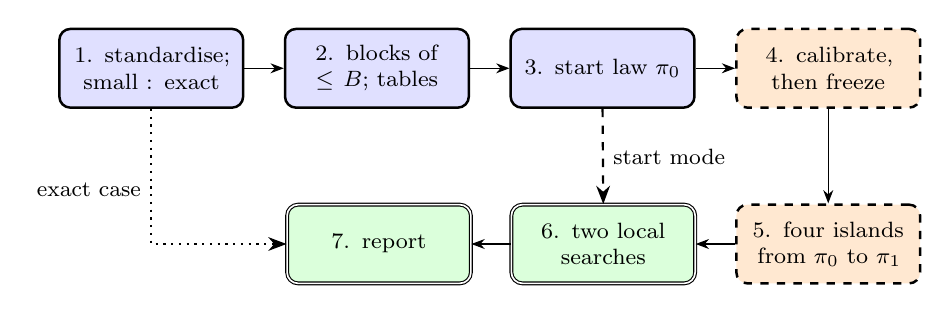
\begin{tikzpicture}[node distance=5mm, every node/.style={font=\footnotesize},
  box/.style={draw, rounded corners, align=center, minimum height=10mm, text width=21mm},
  exact/.style={box, fill=blue!12, line width=0.9pt}, stoch/.style={box, fill=orange!18, dashed, line width=0.9pt},
  det/.style={box, fill=green!14, double}]
\node[exact] (pre) {1. standardise;\\ small $\Om$: exact};
\node[exact, right=of pre] (blk) {2. blocks of\\ $\le B$; tables};
\node[exact, right=of blk] (start) {3. start law $\pi_0$};
\node[stoch, right=of start] (cal) {4. calibrate,\\ then freeze};
\node[stoch, below=12mm of cal] (smc) {5. four islands\\ from $\pi_0$ to $\pi_1$};
\node[det, left=of smc] (ls) {6. two local\\ searches};
\node[det, left=of ls] (out) {7. report};
\draw[-{Stealth}] (pre)--(blk); \draw[-{Stealth}] (blk)--(start); \draw[-{Stealth}] (start)--(cal);
\draw[-{Stealth}] (cal)--(smc); \draw[-{Stealth}] (smc)--(ls); \draw[-{Stealth}] (ls)--(out);
\draw[-{Stealth}, dashed, thick] (start.south) -- node[right, pos=0.5]{start mode $\tSz$} (ls.north);
\draw[-{Stealth}, dotted, thick] (pre.south) |- node[left, pos=0.3]{exact case} (out.west);
\end{tikzpicture}
\caption{The stages of a run. Exact computations: solid boxes (1--3). Random: dashed boxes (4--5). Deterministic given
their inputs: double boxes (6--7). When $\Om$ is small the run goes from stage~1 straight to the report (dotted). The
second local search starts from the start mode and does not depend on the particles (dashed arrow).}
\label{fig:pipeline}
\end{figure}

\paragraph{Stage 1: inputs, the exact case and the check before the run.} The inputs are \emph{valid} when $n\ge3$, at
least one predictor is given and every entry is finite; the seed is an integer in $[1,2^{31}-1]$. Invalid inputs stop the
run. With $N_0:=\max(2500,n,p)$ and $\Nc_0:=\lceil512N_0/2500\rceil$, if $\abs{\Om}\le(5\Nc_0+4N_0)\,p$ the method scores every model
and computes everything exactly. Otherwise it estimates the memory the run will need and the worst-case time of the local search from the start
mode, and stops with status \texttt{resource\_limit} if the
estimate exceeds the allocation (8\,GiB and 24 hours by default).

\paragraph{Stage 2: blocks and block tables.} The method partitions the predictors into blocks $C_1,\dots,C_J$ of at most
$B:=\min(\lfloor\sqrt n\rfloor,\lfloor\sqrt p\rfloor,16)$ predictors, by complete-linkage clustering on $1-\abs{\hat r_{jl}}$,
cutting the tree top-down until every cluster fits and packing whole clusters into blocks in leaf order. The partition is a
deterministic function of $X$, and correlated predictors tend to share a block. Within each block it scores every subset
$U$ with $\abs{U}\le K$ and stores the \emph{block table} $h_k(U):=m(U)/m(\emptyset)$, with $h_k(\emptyset)=1$; a block has
at most $2^{16}$ subsets. It also builds a \emph{neighbour graph} of correlated predictors for the swap moves
(Appendix~\ref{app:params}).

\paragraph{Stage 3: the start law and the start mode.} The start law multiplies the size prior by the block tables,
\begin{equation}\label{eq:startlaw}
  \pi_0(S)=\frac{\gamma_0(S)}{\bar Z_0},\qquad \gamma_0(S):=\frac{w(\abs{S})}{\bar w_K}\prod_{k=1}^J h_k(S\cap C_k),\qquad
  \bar Z_0:=\sum_{S\in\Om}\gamma_0(S):
\end{equation}
the posterior one would have if the marginal likelihood, relative to the empty model, split into independent block
contributions. It sees every interaction within a block and none between blocks. A recursion over model sizes, combining
the blocks one at a time, computes $\bar Z_0$ exactly and gives an exact sampler for $\pi_0$ (draw the total size, then
the size of each block backwards, then a subset of each block). The \emph{start mode} $\tSz$ is a maximiser of $\pi_0$,
computed by the same recursion with maxima: the smallest size among the maximisers, then the lexicographically smallest
set. The posterior and the start law differ by the \emph{discrepancy}
$\Delta(S):=\log\{m(S)/m(\emptyset)\}-\sum_k\log h_k(S\cap C_k)$, the part of the log marginal likelihood that comes from
interactions between blocks: $\gamma_0(S)e^{\Delta(S)}=e^{F(S)}/m(\emptyset)$.

\paragraph{Stages 4 and 5: the sampler.} The sampler moves through the distributions
\begin{equation}\label{eq:path}
  \pi_\xi\ \propto\ \gamma_0\,e^{\xi\Delta},\qquad 0\le\xi\le1,
\end{equation}
from the start law ($\xi=0$) to the posterior ($\xi=1$), along a grid of temperatures $0=\grid0<\dots<\grid{\Ts}=1$ fixed
by the calibration. An island of $N$ particles starts from $N$ independent draws from $\pi_0$. At each step $t$ it
\begin{enumerate}[label=(\alph*),leftmargin=2em,itemsep=0pt,topsep=2pt]
  \item \emph{reweights} particle $v$ by $\omega^{(t)}_v:=\exp\{(\grid t-\grid{t-1})\Delta(S_v)\}$;
  \item \emph{resamples} the particles multinomially, in proportion to these weights;
  \item \emph{moves} every particle by one round of Markov moves that leave $\pi_{\grid t}$ invariant.
\end{enumerate}
A round is an inclusion update (Gibbs) for each predictor, one uniform swap, $B$ swaps along the neighbour graph, and one
independence move that proposes a fresh draw from $\pi_0$. At $\xi=1$ it runs $\Lbi:=\max(4,\lceil\log_2(n+1)\rceil)$ burn-in rounds
and four measured rounds. The island's inclusion-probability estimate $\PIPhat_{r,j}$ averages, over particles and measured
rounds, the conditional inclusion probability of the Gibbs update rather than the 0/1 indicator; its evidence estimate is
$\Zhat_r:=m(\emptyset)\,\bar Z_0\prod_{t=1}^{\Ts}\{N^{-1}\sum_v\omega^{(t)}_v\}$, the exact normaliser of the start law times
the product of the average reweighting factors.

The \emph{calibration} (stage 4) chooses the grid and the effort before the final run, from one pilot island and a few
rounds of four short diagnostic islands; the grid refines the pilot's temperatures so that each step keeps an
effective-sample-size fraction, computed on a set of candidate models, of at least $0.90$. The calibration starts at
tier $i=0$ and moves at most once to tier $i=1$, which multiplies all particle numbers by four, when one of its
diagnostics fires (Appendix~\ref{sec:supp-cal} gives the full procedure). Three facts are all that the results use: the calibration's outcome is a function of the data and of its own
random numbers; it is \emph{frozen} before the final run draws any random number; and it \emph{succeeds} when it freezes a
grid, by its main construction or a fallback (otherwise the run stops without estimates). The \emph{final run} (stage 5)
consists of four independent \emph{islands} of $N_i=4^iN_0$ particles at the frozen tier $i$, on the frozen grid, each with
its own random stream.

\paragraph{Stage 6: the local searches.} Two models are \emph{neighbours} if one comes from the other by deleting a
predictor, adding one (while the size is below $K$), or swapping a member for a non-member. A local search scans every
neighbour of the current model and moves to the best one (ties broken lexicographically) if its log score is strictly
higher, for at most a capped number of moves. It stops at the first scan with no strict improvement and \emph{certifies}
its end point; after its last allowed move it scans once more, and if a neighbour still improves it stops there,
uncertified. Two searches run after the islands: from the best model found so far, with move cap
$\ell_n:=\lceil\log_2(n+p+1)\rceil$; and from the start mode $\tSz$, with move cap $\ell_n+\abs{\tSz}$.

\subsection{What a run reports}\label{sec:outputs-method}

A run either \emph{produces output}, with status ``exact'' (enumeration) or ``completed'' (sampler; a \emph{completed
run}), or stops without estimates. A run stopped by its time guard reports status \texttt{resource\_limit} and returns no
estimates; anything else such a run returns is flagged incomplete, and the results do not cover it. (A constant
response, or no retained predictor, stops the run with the empty model; invalid inputs stop it with no model.) The method records every model
it scores; the \emph{reported model} $\Shat$ is the best of them by log score (exact ties to the smaller model, then
lexicographically). It is \emph{certified} when the method enumerated $\Om$, or when $\Shat$ ends a local search whose last
scan found no strict improvement. An exact run reports $\Shat$, every $\PIP_j$, the median probability model and $\log Z$.
A completed run pools its islands with equal weights,
\begin{equation}\label{eq:pool}
  \PIPhat_j:=\frac14\sum_{r=1}^4\PIPhat_{r,j},\qquad \Zhat:=\frac14\sum_{r=1}^4\Zhat_r,
\end{equation}
and reports $\Shat$, the $\PIPhat_j$, the estimated median probability model $\MPMhat:=\{j:\PIPhat_j>1/2\}$, $\log\Zhat$
with a one-sided $95\%$ lower bound $\log(0.05\,\Zhat)$ for $\log Z$ (Appendix~\ref{app:params}), a flag saying whether
$\Shat$ is certified, and a list $\mathcal T$ of at most $40p+1$ models with their log scores, the best among those it scored. Islands are not
weighted by their evidence estimates. Diagnostics, which never change an output, are listed in
Appendix~\ref{app:params}.

\subsection{The constants}\label{sec:constants}

Table~\ref{tab:params} lists the constants of the method that the results use or that a reader needs. Appendix~\ref{app:params}
gives all of them, with their code locations.

\begin{table}[ht]
\centering\small
\setlength{\tabcolsep}{4pt}
\caption{The main constants of the method. Every one is a numerical constant or a function of $(n,p)$; the example
column uses $n=200$, $p=10^4$.}\label{tab:params}
\begin{tabular}{@{}>{\raggedright\arraybackslash}p{0.34\linewidth}l>{\raggedright\arraybackslash}p{0.3\linewidth}r@{}}
\toprule
Constant & Symbol & Value & Example \\
\midrule
size cap & $K$ & $\min(p,\lfloor n/2\rfloor)$ & 100 \\
model prior & $w(k)$ & $\tfrac12/\binom{2p-1}{k}$, renormalised to $\Om$ & \\
coefficient prior scale; ridge & $g$ & $n$; unit ridge & 200 \\
inverse-gamma shape and scale & $a_0,b_0$ & $0.01$, $0.01$ & \\
block size cap & $B$ & $\min(\lfloor\sqrt n\rfloor,\lfloor\sqrt p\rfloor,16)$ & 14 \\
particles per island (tier $i$) & $N_i$ & $4^i\max(2500,n,p)$ & $10^4$; $4\cdot10^4$ \\
islands; measured rounds & & $4$; $4$ & \\
burn-in rounds at $\xi=1$ & $\Lbi$ & $\max(4,\lceil\log_2(n+1)\rceil)$ & 8 \\
moves per round & & $p$ inclusion updates, $1$ uniform swap, $B$ neighbour swaps, $1$ independence move & 10,016 \\
calibration grid target & & restricted effective-sample-size fraction $\ge0.90$ & \\
exact-case threshold & & enumerate if $\abs{\Om}\le(5\Nc_0+4N_0)\,p$ & $5.0\times10^8$ \\
base move cap & $\ell_n$ & $\lceil\log_2(n+p+1)\rceil$ & 14 \\
move cap from the start mode & & $\ell_n+\abs{\tSz}$ & \\
returned list & $\mathcal T$ & best $40p+1$ models by $F$ & 400,001 \\
pooling of islands & & equal weights & \\
\bottomrule
\end{tabular}
\end{table}

\subsection{What the results use from the method}\label{sec:conventions}

The results of Section~\ref{sec:results} use five objects of a run: the start law and its mode (stage 3), the reported
model and its certification (stages 6--7), the pooled estimates~\eqref{eq:pool}, the returned list $\mathcal T$, and the
event $\Acal$ that the method uses the sampler and its calibration succeeds. A run in $\Acal$ may still stop later, at
its time guard; every completed run lies in $\Acal$. They also
use three conventions, which fix what ``the method'' means and idealise the computer; they are not statistical
assumptions, and Appendix~\ref{app:params} lists them in full. Exact arithmetic and ideal random numbers are also
presupposed by Song and Liang's statements about their own sampler (their supplement, pp.~9--10, 12--13).
\begin{itemize}[leftmargin=1.5em,itemsep=1pt]
  \item \phantomsection\label{asm:C1}\emph{Convention \as{C1} (the method):} exact arithmetic, the default configuration,
    valid inputs and seed. A run that meets it is \emph{admissible}; a sample size $n$ is admissible if some data set of
    that size is valid. Statements hold for every valid seed and every outcome of the calibration.
  \item \phantomsection\label{asm:C2p}\emph{Convention \as{C2p} (delivery):} an idealised
    machine that never overflows or fails, ideal random numbers, an allocation of at least the memory and time that the method's own polynomial
    requirement formulas require, and the code's two fixed integer limits on the move caps lifted (see the remark after
    Theorem~\ref{thm:reported}).
  \item \phantomsection\label{asm:C3}\emph{Convention \as{C3} (sampler):} exact arithmetic, ideal random numbers
    independent of the data and of the calibration, an exact start sampler, and Markov moves that do what their definitions
    say.
\end{itemize}

% =====================================================================================================
\section{Main results}\label{sec:results}

Table~\ref{tab:results} lists the five results. Each is stated in the same format: what it says in words, why it
matters, the statement, its assumptions with the place in Section~\ref{sec:assumptions} where each one is judged, a
one-line scope (which of our designs are inside; Section~\ref{sec:who-outside}), and a status note.

\begin{table}[!t]
\centering\footnotesize
\setlength{\tabcolsep}{3.5pt}
\renewcommand{\arraystretch}{1.12}
\caption{The five results. Statuses are those of the project's registry as frozen at \texttt{theory-v2026-11-freeze};
every check is independent of the author.}\label{tab:results}
\begin{tabular}{@{}>{\raggedright\arraybackslash}p{0.17\linewidth}>{\raggedright\arraybackslash}p{0.3\linewidth}>{\raggedright\arraybackslash}p{0.26\linewidth}>{\raggedright\arraybackslash}p{0.2\linewidth}@{}}
\toprule
Result & In words & Key assumptions & Status \\
\midrule
1.~The posterior finds the true model (Thms~\ref{thm:post-random}, \ref{thm:post-fixed}) &
The posterior mass outside the true model is of order $\rn$; the highest posterior and median probability models equal
the true model with probability tending to one. &
Gaussian linear model; $p\le n^A$; a fixed number of fixed nonzero coefficients (for a fixed design, a beta-min
condition instead); an eigenvalue floor on sets of $O(\log n)$ predictors. &
Proved and checked; the fixed-design expectation bound rests on one supporting result not yet checked. \\
2.~It finds the true distribution (Thm~\ref{thm:dist}) &
The posterior contracts around the true conditional law of the response, at radius of order $\rn$ in the Hellinger distance. &
i.i.d.\ observations; sparse Gaussian linear model; light-tailed predictors; no near-exact collinearity; no predictor with an unbounded
signal; no lower bound on the coefficients. &
Proved and checked. \\
3.~The method, as coded, reports the true model (Thm~\ref{thm:reported}) &
With probability tending to one, every run that produces output reports exactly the true model, whatever its seed. &
Gaussian rows; fixed signals; every true predictor visible (its signal does not cancel against any $15$ others); the predictors that can imitate the signal are few,
and local. &
Proved and checked; no open condition. \\
4.~The run's estimates (Prop.~\ref{prop:unbiased}, Thm~\ref{thm:outputs}) &
The evidence estimate is unbiased on every design. On designs without leakage the errors of the reported inclusion
probabilities, median model and evidence estimate (relative and log error), multiplied by the indicator that the sampler
is used and its calibration succeeds, tend to zero. &
Unbiasedness: none on the design. Consistency: Gaussian rows, fixed signals, visibility, and no null predictor
correlated with a true one beyond order $n^{-1/2}$, even given $15$ others. &
Unbiasedness: proved and checked. Consistency: proved and checked, conditional on two results on the coded sampler that
are themselves proved under named premises and checked. \\
5.~The rate cannot be improved (Rem.~\ref{rem:sharp}) &
For true models of at most $\min(K-1,p/2)$ predictors no design gives a rate faster than $n^{-1/2}$; on two
families of designs the expected posterior miss is at least of order $\rn$, and on orthogonal designs of exactly that
order. &
None for the first part; orthogonal or Gaussian null predictors for the second. &
Proved and checked; the exact order on orthogonal designs uses the fixed-design expectation bound and has its
status. \\
\bottomrule
\end{tabular}
\end{table}

\subsection{Shared assumptions}\label{sec:standing}

The assumptions below are used by several results; the others are stated with the result that uses them. Two words recur
in Results~3 and~4. A true predictor is \emph{visible} if its signal does not cancel against any $15$ other predictors (the
method's blocks hold at most $16$); a null predictor \emph{leaks} if, given up to $15$ others, it can imitate part of a
true predictor's signal (Example~\ref{ex:leak}).

\begin{assumption}{GL}{Gaussian linear model}
The data follow~\eqref{eq:model}, with a fixed noise variance $\sigs^2>0$ and noise independent of the design. \hfill [\SA{all}]
\end{assumption}

\begin{assumption}{DIM}{Dimension}
$2\le p\le n^A$ for a fixed $A\ge1$. \hfill [\SA{all}]
\end{assumption}

\begin{assumption}{SP}{Sparsity}
The true model size $\sz\ge1$ is fixed. \hfill [\SA{all}]
\end{assumption}

\begin{assumption}{GR}{Gaussian rows}
The rows of $\Xr$ are i.i.d.\ $\Normal_p(m_n,\Sig)$, where $\Sig$ is a correlation matrix. \hfill [\SA{post}]
\end{assumption}

\begin{assumption}{EFS}{Population eigenvalue floor}
$\lmin(\Sigma_{n,S})\ge\varphi^2$ for every $S$ with $\abs{S}\le5(A+1)(\sz+1)\log n$, for a fixed $\varphi\in(0,1]$ (for
instance, $\lmin(\Sig)\ge\varphi^2$). \hfill [\SA{post}]
\end{assumption}


% =====================================================================================================
\subsection{Result 1: the posterior finds the true model}\label{sec:model-result}

\inwords{If the true model is small and its coefficients are fixed and nonzero, and no small group of predictors is
collinear, then the posterior puts all but a fraction of order $\rn$ of its mass on the true model. The highest posterior
model and the median probability model then equal the true model with probability tending to one, and every inclusion
probability is within order $\rn$ of $1$ for a true predictor and of $0$ for a null one. We state this first for Gaussian
rows, the case of our simulation designs, and then for a fixed design, with conditions on the sample.}

\why{It is the basic guarantee of a Bayesian selection method, here for the prior exactly as the software sets it: with
enough data the posterior points to the right predictors, and its inclusion probabilities can be read as near-certain
inclusion or exclusion.}

\begin{assumption}{FSb}{Fixed signals, raw scale}
$b_{\mathrm{lo}}\le\abs{\beta^*_j}\le b_{\mathrm{hi}}$ for every $j\in\Sz$, with fixed $0<b_{\mathrm{lo}}\le b_{\mathrm{hi}}<\infty$. \hfill [\SA{post}]
\end{assumption}

\begin{theorem}[Posterior concentration, random Gaussian design]\label{thm:post-random}
Assume \as{GL}, \as{DIM}, \as{SP}, \as{GR}, \as{FSb} and \as{EFS}. Then, under the joint law of the design and the noise,
\begin{gather}
  1-\pis{\Sz}=\OP\Big(\sqrt{\frac{\log n}{n}}\Big),\qquad \P\big(\HPM=\MPM=\Sz\big)\to1,\label{eq:post-random}\\
  \max_{j\in\set{p}}\big|\PIP_j-\ind{j\in\Sz}\big|=\OP\Big(\sqrt{\frac{\log n}{n}}\Big).\nonumber
\end{gather}
\end{theorem}

\asmlist{(1)~\as{GL} Gaussian linear model; (2)~\as{DIM} $p\le n^A$; (3)~\as{SP} fixed $\sz$ [\SA{all}]; (4)~\as{GR}
Gaussian rows; (5)~\as{FSb} fixed nonzero coefficients; (6)~\as{EFS} population eigenvalue floor on sets of
$O(\log n)$ predictors [\SA{post}].}
\scope{Every design of our simulation studies, strong common factors included.}

\status{\textbf{Proved and independently checked}: the fixed-design result it rests on (Theorem~\ref{thm:post-fixed},
in-probability form) and the transfer from population to sample conditions are each proved and independently checked.
Registry: Appendix~\ref{app:status}, row 1.2.}

No upper bound on the eigenvalues of $\Sig$ is needed, so strong common factors are allowed, and $p\gg n$ is allowed. In
primitive terms: a Gaussian linear model with i.i.d.\ Gaussian rows whose correlation matrix has smallest eigenvalue bounded below, a fixed number of
fixed nonzero coefficients and $p\le n^A$ suffice.

\paragraph{Fixed design.} The same conclusions hold for a deterministic design under conditions on the sample. They
use four more assumptions.

\begin{assumption}{BC}{Bounded coefficients}
$\max_{j}\abs{\theta^*_j}\le\bar\theta$ for a fixed $\bar\theta<\infty$. \hfill [\SA{post}]
\end{assumption}

\begin{assumption}{EF}{Eigenvalue floor on sets of bounded size}
$\lmin(\Rhat_S)\ge\varphi_0^2$ for every model $S$ with $\abs{S}\le2(A+1)\sz+2$, for a fixed $\varphi_0\in(0,1]$. \hfill [\SA{post}]
\end{assumption}

\begin{assumption}{NC}{No near-exact collinearity among sets of logarithmic size}
$\lmin(G_S)\ge g_0$ for every model $S$ with $\abs{S}\le3(A+1)(\sz+1)\log n$, for a fixed $g_0>0$; on the correlation
scale, a floor $g_0/(n-1)$ that vanishes as $n$ grows. \hfill [\SA{post}]
\end{assumption}

\begin{assumption}{BM}{Beta-min}
Either (a) $\tmin\ge C_\beta\,\sigs\rn$ with a fixed $C_\beta>0$ such that $C_\beta^2\varphi_0^2>c_0(\sz,A)$, an explicit
constant (Appendix~\ref{app:constants}); or (b) $\tmin\sqrt{n/\log n}\to\infty$. \hfill [\SA{post}]
\end{assumption}

\begin{theorem}[Posterior concentration, fixed design]\label{thm:post-fixed}
Let the design be fixed and assume \as{GL}, \as{DIM}, \as{SP}, \as{BC}, \as{EF}, \as{NC} and \as{BM}. Then, along every
sequence that satisfies these assumptions,
\begin{equation}\label{eq:post-op}
  \max_{j\in\set{p}}\big|\PIP_j-\ind{j\in\Sz}\big|\ \le\ 1-\pis{\Sz}\ =\ \OP\Big(\sqrt{\frac{\log n}{n}}\Big),\qquad
  \P\big(\HPM=\MPM=\Sz\big)\to1 .
\end{equation}
Moreover, there are $n_0$ and $C_{\mathrm E}$, depending only on $(\sz,A,\sigs^2,\bar\theta,\varphi_0,g_0,C_\beta)$, such that for
every $n\ge n_0$ and every design and $\tstar$ that satisfy the assumptions at that $n$,
\begin{equation}\label{eq:post-exp}
  \E\big[1-\pis{\Sz}\big]\ \le\ C_{\mathrm E}\sqrt{\frac{\log n}{n}},\qquad \P\big(\HPM=\MPM=\Sz\big)\ \ge\ 1-4C_{\mathrm E}\sqrt{\frac{\log n}{n}} .
\end{equation}
The expectation is over the noise, with the design fixed. Under form (b) of \as{BM}, $n_0$ also depends on how fast
$\tmin\sqrt{n/\log n}$ diverges.
\end{theorem}

\asmlist{(1)--(3)~\as{GL}, \as{DIM}, \as{SP} [\SA{all}]; (4)~\as{BC} bounded coefficients; (5)~\as{EF} eigenvalue floor
on sets of bounded size; (6)~\as{NC} no near-exact collinearity; (7)~\as{BM} beta-min [\SA{post}].}

\status{The in-probability conclusions~\eqref{eq:post-op}: \textbf{proved and independently checked}. The expectation
bound~\eqref{eq:post-exp}: \textbf{proved and checked, conditional on one supporting result} (a proposition giving a lower
bound on the posterior miss) \textbf{that is proved but not yet independently checked}; its other input, a lemma bounding
the tail of the posterior model size, is now independently checked. Registry: Appendix~\ref{app:status}, row 1.1.}

\subsection{Result 2: the posterior finds the true distribution}\label{sec:distribution}

\inwords{Suppose the observations are i.i.d., the response follows a sparse Gaussian linear model, the predictors have light
tails, no small group of predictors is almost exactly collinear, and no single predictor carries an unbounded signal.
Then, for every large enough level $M$, with probability at least $1-n^{-c_{\mathrm H}M}$ the posterior puts mass at
most $n^{-c_{\mathrm H}M}$ on conditional laws of the response farther than $\sqrt{M\log n/n}$ from the true one, in the
Hellinger distance. No
lower bound on the coefficients is needed.}

\why{The posterior describes the response correctly even when some true predictors are too weak to be selected, so
prediction does not depend on perfect selection.}

\paragraph{Setting.} In this section only, the observations are $n$ i.i.d.\ copies $(x^{(i)},y^{(i)})$ of a pair $(x,y)$,
with $x\in\R^{\praw}$ the vector of all observed predictors; $\Dn$ is the data set, $\P^*$ its law, and the method runs on
the predictors that are not constant in the sample. The posterior is not defined if fewer than two predictors remain or
the response is constant in the sample; such data sets are counted in the exceptional event of the theorem. A posterior draw $(S,\beta,\sigma^2)$, mapped back to the original
units, defines the conditional law $\Normal(\bar y+(x-\bar x)^\top\beta,\sigma^2)$ of $y$ given $x$; the law of $x$ is not
estimated. Let $f$ be the joint density of $(x,y)$ with $x$ from its true law and $y\mid x$ from this fitted law, and $f^*$
the true joint density; then $d_H(f,f^*):=(1-\int\sqrt{ff^*})^{1/2}$ is the Hellinger distance between the fitted and the true conditional
laws, averaged over a new $x$. $\Pi(\cdot\mid\Dn)$ is the posterior of $(S,\beta,\sigma^2)$, and
$\zeta_j:=(x_j-\E x_j)/\sd(x_j)$. Fix a \emph{level} $M\ge1$; the \emph{window} $q_n:=\min\{\praw,\lceil C_qM\log
n\rceil\}$, $C_q:=2(s(A+2)+4)/\log2$, is the largest number of predictors the conditions constrain jointly.

\begin{localassumption}[Distribution-level setting]\label{asm:dist}
The integer $s\ge0$ and the constants $A\ge1$, $L\ge1$, $c_\psi>0$ and $\bar b>0$ are fixed.
\begin{asmitems}
  \item\label{asm:dist-model} \emph{Gaussian linear model for i.i.d.\ pairs.} $y=\alpha^*+x^\top\bstar+\varepsilon$ with
    $\varepsilon\sim\Normal(0,\sigs^2)$, $\sigs^2>0$, independent of $x$; $\alpha^*$, $\bstar$, $\sigs$ and the law of $x$ may
    depend on $n$.
  \item\label{asm:dist-sparse} \emph{Sparsity and dimension.} At most $s$ coordinates of $\bstar$ are nonzero, and
    $2\le\praw\le n^A$.
  \item\label{asm:dist-subg} \emph{Sub-Gaussian predictors on sparse directions.} Every predictor has positive variance,
    and $\E\exp(\lambda u^\top\zeta)\le\exp\big(L^2\lambda^2\Var(u^\top\zeta)/2\big)$ for every $\lambda\in\R$ and every
    $u\in\R^{\praw}$ with at most $q_n$ nonzero entries.
  \item\label{asm:dist-nec} \emph{No near-exact collinearity.} $\lmin(\Corr(x_T))\ge c_\psi/n$ for every set $T$ of at
    most $q_n$ predictors.
  \item\label{asm:dist-bs} \emph{Bounded signal.} $\abs{\beta^*_j}\sd(x_j)\le\bar b\,\sigs$ for every $j$.
\end{asmitems}
\end{localassumption}

\begin{theorem}[Distribution-level consistency]\label{thm:dist}
There are constants $c_{\mathrm H}>0$, $M_0$ and $n_0$, depending only on $(s,A,L,c_\psi,\bar b)$, such that the following
holds. Fix a level $M\ge M_0$ and assume Assumption~\ref{asm:dist}, with the window $q_n$ of this $M$. Then for every
$n\ge n_0$ with $\sqrt n/\log n\ge M$,
\begin{equation}\label{eq:dist-i}
  \P^*\Big[\,\Pi\Big(d_H(f,f^*)>\sqrt{M\log n/n}\ \Big|\ \Dn\Big)>n^{-c_{\mathrm H} M}\Big]\ \le\ n^{-c_{\mathrm H} M}.
\end{equation}
\end{theorem}

\asmlist{(1)~Assumption~\ref{asm:dist}\ref{asm:dist-model}: Gaussian linear model [\SA{all}]; (2)~\ref{asm:dist-sparse}:
sparsity and $\praw\le n^A$ [\SA{all}]; (3)~\ref{asm:dist-subg}: light-tailed predictors [\SA{post}, law of the rows];
(4)~\ref{asm:dist-nec}: no near-exact collinearity [\SA{post}]; (5)~\ref{asm:dist-bs}: bounded signal [\SA{post}, signal
size].}

\scope{Every design of our simulation studies (Section~\ref{sec:who-outside}).}

\status{\textbf{Proved and independently checked}. Registry: Appendix~\ref{app:status}, row 2.1.}

\begin{remark}[On the assumptions]\label{rem:dist-asm}
No beta-min condition and no fixed lower bound on eigenvalues are assumed. Jointly Gaussian predictors satisfy Assumption~\ref{asm:dist}\ref{asm:dist-subg} with $L=1$, and every correlation matrix whose $q_n\times q_n$
principal blocks have smallest eigenvalue at least a fixed $\psi>0$ satisfies Assumption~\ref{asm:dist}\ref{asm:dist-nec}
for all large $n$. Condition~\ref{asm:dist-nec} keeps the Occam factor of each extra predictor in force; without it the
radius grows by one factor $\sqrt{\log(\praw\vee n)}$ (Proposition~\ref{prop:dist}). The same statement holds for every
level $M$ up to $\sqrt n/\log n$, with the same constants. It also carries over to the list of models that a completed run returns,
when that list holds posterior mass at least $n^{-c_{\mathrm H}M/2}$, a condition the run does not check
(Corollary~\ref{cor:dist-output}).
\end{remark}

% =====================================================================================================
\subsection{Result 3: the method, as coded, reports the true model}\label{sec:reported}

\inwords{If every true predictor is visible to a block-by-block search, the predictors that can imitate the signal form a
set $Q$ of at most $n^b$ predictors with $b<\tfrac12$, and regressions within $Q$ are local, then there is an event,
determined by the data alone and of probability tending to one, on which every run that produces output reports exactly
the true model, whatever its seed and the outcome of its calibration. The mechanism is that of
Example~\ref{ex:leak}: the start mode holds the true predictors and possibly some members of $Q$, and the local search
from the start mode deletes the spurious ones.}

\why{It is a guarantee about what the software reports, at the effort its own calibration chooses and for every seed, not only
about the posterior it targets.}

\paragraph{How the signal looks to a block-by-block method.} The start law sees interactions within blocks of at most
$16$ predictors only, so the conditions of this section are about partial covariances given at most $15$ other
predictors. With $W\sim\Normal_p(0,\Sig)$, $\Cov(W_j,W_l\mid W_U)$ is the partial covariance given $(W_k)_{k\in U}$, and
$\bar\beta_{U,l}:=\Sigma_{n,UU}^{-1}\Sigma_{n,Ul}$ is the population regression coefficient of $W_l$ on $W_U$, padded
with zeros to a vector indexed by a larger set when needed. A
\emph{leakage set} is a deterministic $Q$ with $\Sz\subseteq Q\subseteq\set{p}$ that contains every predictor able to
imitate part of the signal; its \emph{lattice} $\Lat(Q):=\{T:\Sz\subseteq T\subseteq Q\}$ is the set of models between the
true model and $Q$. The signal is fixed on the scale the method sees:

\begin{assumption}{FSt}{Fixed signals, standardised scale}
$\yr=\alpha\one+X\tstar+\varepsilon$ with $\varepsilon\sim\Normal_n(0,\sigs^2I_n)$, a fixed $\sigs^2>0$, noise independent
of $\Xr$, a deterministic $\tstar$, $\sz\ge1$ fixed, and $\theta_{\mathrm{lo}}\le\abs{\theta^*_j}\le\theta_{\mathrm{hi}}$ for
$j\in\Sz$, with fixed $0<\theta_{\mathrm{lo}}\le\theta_{\mathrm{hi}}$. \hfill [\SA{post}]
\end{assumption}

\begin{assumption}{V}{Visibility}
For every $j\in\Sz$ and every $U\not\ni j$ with $\abs{U}\le15$, $\abs{\Cov(W_j,W^\top\tstar\mid W_U)}\ge a$, for a fixed
$a>0$. \hfill [\SA{rm}]
\end{assumption}

In \as{FSt} the raw coefficients $\bstar=D^{-1}\tstar$ depend on the design; \as{FSt} takes the place of \as{GL} and \as{SP}
in Results~3 and~4.

Visibility excludes masking: if two true predictors with coefficients $1$ and $-1$ have correlation $\rho$, the
signal of each, given nothing, is $1-\rho$, and it vanishes as $\rho\to1$. A null predictor whose correlation with
a true one stays fixed must belong to the leakage set $Q$, as predictor $5$ does in Example~\ref{ex:leak}.

Fix $b\in(0,\tfrac12)$ and $b_H>0$ with $15b_H+b<\tfrac12$.

\begin{localassumption}[Polynomial leakage set with local regressions]\label{asm:reported}
\begin{asmitems}
  \item\label{asm:rr-leak} \emph{Leakage set.} There is a deterministic $Q\supseteq\Sz$ with $\abs{Q}\le n^b$ and, for
    large $n$, $\abs{Q}\le K$ and ($Q=\set{p}$ or $K\ge2\abs{Q}+32\sz+1$), such that: (i) \emph{no leak outside $Q$:}
    there is a deterministic $\varpi_n$ with $\varpi_n\sqrt{n/\log n}\to0$ such that
    $\abs{\Cov(W_l,W_j\mid W_U)}\le\varpi_n$ for all $l\notin Q$, $j\in\Sz\setminus U$ and $\abs{U}\le15$; and (ii)
    \emph{locality:} there is a deterministic $r_n\to0$, and every $l\notin Q$ has a deterministic
    $\Hl_l\supseteq\{l\}\cup\Sz$ with $\abs{\Hl_l}\le n^{b_H}$, such that for all $l\notin Q$, all $U\not\ni l$ with
    $\abs{U}\le15$ and $U_0:=U\cap\Hl_l$: $\abs{\Cov(W_l,W_v\mid W_{U_0})}\le r_n$ and
    $\abs{\Cov(W_j,W_v\mid W_{U_0})}\le r_n$ for all $v\in U\setminus\Hl_l$ and $j\in\Sz\setminus U_0$.
  \item\label{asm:rr-floor} \emph{Floor on the leakage set.} $\lmin(\Sigma_{n,Q\cup\{l\}})\ge\varphi^2$ for every
    $l\in\set{p}$, with $\varphi$ as in \as{EFS}.
  \item\label{asm:rr-local} \emph{Local regressions within the leakage set.} There are deterministic sequences
    $d_n=o(\log n)$ and $L_n$, and for every $l\in\set{p}$ a deterministic $N_l\subseteq Q\setminus\{l\}$ with
    $\abs{N_l}\le d_n$, such that $\norm{\bar\beta_{T,l}-\bar\beta_{T\cap N_l,l}}_1\le L_n$ for every $T\in\Lat(Q)$ with
    $l\notin T$, where $L_n\to0$ and $L_n^2\log(\abs{Q}+1)=o(\log n)$.
\end{asmitems}
\end{localassumption}

In~(a), $32\sz=2\cdot16\sz$, with $16$ the method's block-size cap: with probability tending to one the start mode has at
most $2(\abs{Q}+16\sz)$ predictors, so this condition leaves room to add a missing true predictor to it.

\begin{theorem}[The reported model equals the true model]\label{thm:reported}
Let $\Sig$ be positive definite and assume \as{GR}, \as{DIM}, \as{FSt}, \as{V}, \as{EFS}, Assumption~\ref{asm:reported}
and Convention~\as{C1}. Then, under the joint law of the design and the noise, there are data events $\mathcal G_n$ with
$\P(\mathcal G_n)\to1$ on which \emph{every} admissible run that produces output reports $\Shat=\Sz$, whatever its seed and the
outcome of its internal calibration. In particular,
\begin{equation}\label{eq:reported}
  \P(\text{the run produces output and }\Shat\neq\Sz)\to0 .
\end{equation}
If moreover Convention~\as{C2p} holds, then
\begin{equation}\label{eq:delivery}
  \P(\text{the run produces output})=1\ \ \text{for every admissible }n\ge3,\qquad \P(\Shat=\Sz)\to1 .
\end{equation}
\end{theorem}

Convention~\as{C2p} lifts two integer limits of the code; in the default configuration neither can be reached on any input
R can represent ($n,\praw\le2^{31}-1$), so this matters only for the form as $n\to\infty$ (Appendix~\ref{app:conventions}).

\asmlist{(1)~\as{GR} Gaussian rows; (2)~\as{DIM} [\SA{all}]; (3)~\as{FSt} fixed signals [\SA{post}]; (4)~\as{V}
visibility [\SA{rm}]; (5)~\as{EFS} population floor [\SA{post}]; (6)~Assumption~\ref{asm:reported}(a) polynomial
leakage set, and (b)--(c) floor and local regressions in it [\SA{rm}]; (7)~Conventions \as{C1}, and \as{C2p} for delivery
(Appendix~\ref{app:conventions}).}

\status{\textbf{Proved and independently checked}, with no open condition: the version proved in the registry is a stronger form of
this statement, and the two code-reading audits that its delivery route takes as hypotheses are independently checked.
The statement that the integer limits of \as{C2p} cannot be reached on any representable input: \textbf{proved and
independently checked}. Registry: Appendix~\ref{app:status}, row 3.1.}

\begin{remark}[On the assumptions]\label{rem:reported}
(i) \emph{Why $b<\tfrac12$.} At model size about $\sqrt n$ the prior-plus-Occam penalty of one more predictor
($\approx\log p+\tfrac12\log n$) stops dominating the best of $p$ noise gains ($\approx\log p$); for larger $b$ the key events of the argument are
expected to fail (a heuristic; whether the conclusion fails is open).
(ii) Designs that satisfy the assumptions include correlation that is local in a metric, and bounded blocks.
\end{remark}

\scope{The independent and locally correlated designs of our studies; not pervasive common factors with $p\gg\sqrt n$
(Section~\ref{sec:who-outside}).}

% =====================================================================================================
\subsection{Result 4: the run's estimates}\label{sec:estimates}

\inwords{The method reports an evidence estimate, pooled inclusion probabilities and the median probability model they
define. Given the calibration, the evidence estimate is unbiased, on every design. If, in addition, the rows are Gaussian, the signals fixed, every true predictor visible, and no
null predictor correlated with a true one beyond order $n^{-1/2}$, even given $15$ others, the reported estimates are
consistent: the errors of the evidence estimate (relative and log error) and of the inclusion probabilities, multiplied
by the indicator that the method uses the sampler and its calibration succeeds, are of order
$n^{-1/2}e^{C_\rho\sqrt{\log n}}=n^{-1/2+o(1)}$; the probability that this event occurs and the median model is wrong tends
to zero, and so does the probability that the run completes and the reported model is wrong.}

\why{The numbers a user reads come with guarantees: the evidence estimate is right on average on every design, and on
designs without leakage, on the event that the calibration succeeds, the reported summaries converge to their targets.}

\subsubsection{Unbiased evidence, on every design}\label{sec:unbiased}

\begin{proposition}[Each island's evidence estimate is unbiased]\label{prop:unbiased}
Under Convention~\as{C3}, given the calibration, each island's evidence estimate $\Zhat_r$ is unbiased for $Z$, for every
design and data set.
\end{proposition}

\asmlist{Convention \as{C3} only; no condition on the design (Appendix~\ref{app:conventions}).}

\status{\textbf{Proved and independently checked}. Registry: Appendix~\ref{app:status}, row 3.5.}

This is the classical unbiasedness of sequential Monte Carlo estimates of normalising constants \citep{DelMoral2004},
established for the method as coded, calibration included: the calibration is frozen before the final run draws its
random numbers. By linearity the equal-weight pooled estimate is then unbiased too: on $\Acal$,
$\E[\Zhat\mid\text{calibration}]=Z$.

\status{Pooled form: \textbf{proved and independently checked}; the frozen-run identities behind both forms are
proved and independently checked against the code of record. Registry: Appendix~\ref{app:status}, row 3.5.}

\subsubsection{Consistent estimates, on designs without leakage}\label{sec:outputs}

\scope{Proposition~\ref{prop:unbiased}: every design. Theorem~\ref{thm:outputs}: only the independent designs of our
studies, since it needs \as{NL} below, no leakage at all (Section~\ref{sec:who-outside}).}

\begin{assumption}{NL}{No leakage, as seen by the start law}
Every null predictor $l\notin\Sz$ has a deterministic \emph{neighbourhood} $\Hl_l\supseteq\{l\}\cup\Sz$ with
$\abs{\Hl_l}\le e^{\kappa_H\sqrt{\log n}}$ for a fixed $\kappa_H$, such that, for every $U\not\ni l$ with $\abs{U}\le15$ and
$U_0:=U\cap\Hl_l$: (i) \emph{no leak:} $\abs{\Cov(W_l,W_j\mid W_{U_0})}\le C_Ln^{-1/2}$ for every $j\in\Sz\setminus U_0$,
with a fixed $C_L$; and (ii) \emph{locality:} $\abs{\Cov(W_l,W_v\mid W_{U_0})}\le r^\circ_n$ and
$\abs{\Cov(W_j,W_v\mid W_{U_0})}\le r^\circ_n$ for every $v\in U\setminus\Hl_l$ and $j\in\Sz\setminus U_0$, where
$r^\circ_n(n\log n)^{1/4}\to0$. \hfill [\SA{pe}]
\end{assumption}

The theorem concerns runs that use the sampler; enumeration is not covered. On the event $\Acal$ of
Section~\ref{sec:conventions}, $\Zhat$, $\PIPhat$ and
$\MPMhat$ denote the pooled values the four islands would produce if the run did not stop; on completed runs they
are the reported values. Let $\rho_n:=n^{-1/2}e^{C_\rho\sqrt{\log n}}$, with $C_\rho$ depending only on the fixed quantities of the
assumptions.

\begin{theorem}[The reported estimates are consistent]\label{thm:outputs}
Assume \as{GR}, \as{DIM} with $p>\sz$, \as{FSt}, \as{EFS}, \as{V}, \as{NL}, and Conventions~\as{C1} and~\as{C3}. Then,
under the joint law of the design, the noise and the method's random numbers,
\begin{gather}
  \ind{\Acal}\Big(\big|\Zhat/Z-1\big|+\big|\log\Zhat-\log Z\big|+\max_{j\in\set{p}}\big|\PIPhat_j-\ind{j\in\Sz}\big|\Big)
    =\OP(\rho_n),\label{eq:outputs-rate}\\
  \P\big(\Acal\cap\{\MPMhat\neq\Sz\}\big)\to0,\qquad \P\big(\text{the run completes and }\Shat\neq\Sz\big)\to0,
    \label{eq:outputs-sel}
\end{gather}
and~\eqref{eq:outputs-rate} also holds for the reported values multiplied by the indicator of a completed run.
\end{theorem}

\asmlist{(1)~\as{GR}, \as{FSt}, \as{EFS}, \as{V} as in Result~3; (2)~\as{DIM} [\SA{all}]; (3)~\as{NL} no leakage
[\SA{pe}]; (4)~Conventions \as{C1}, \as{C3} (Appendix~\ref{app:conventions}).}

\status{\textbf{Proved and checked, conditional on} \samplerconds. Registry: Appendix~\ref{app:status}, row 3.6.}

\begin{remark}[What is not claimed]\label{rem:outputs}
(i) No lower bound on $\P(\Acal)$ is asserted: the statements are about intersections with $\Acal$ or with completion, not
conditional on them.
(ii) The rate $\rho_n$ is the start law's rate; it is slower than the posterior rate $\rn$, by the factor
$e^{C_\rho\sqrt{\log n}}/\sqrt{\log n}$.
(iii) Pooling cannot make things worse: the pooled inclusion probabilities are never farther from the exact ones, in the
largest coordinate, than those of the worst island (proved and checked, conditional on the same two sampler results as
Theorem~\ref{thm:outputs}; registry row 4.1).
\end{remark}

\subsection{Result 5: the rate cannot be improved}\label{sec:sharp}

\inwords{On every design, no model of at most $\min(K-1,p/2)$ predictors has posterior mass closer to one than about
$(\abs{S}+1)/(3\sqrt n)$; on two families of designs the expected posterior miss is at least of order $\rn$. At simulated sizes the posterior spreads over the true model and
its one-predictor extensions.}

\why{It shows that the rate of Result~1 is the right one, and why the posterior is not a point mass at simulated sizes
such as $n=200$.}
\scope{(a) Every design; (b) the witness designs only.}

\begin{remark}[The rate cannot be improved, and what it means at moderate $n$]\label{rem:sharp}
\textup{(a)} \emph{Every design.} For every $n\ge3$, every standardised design with $p\ge2$, every response and every
model $S$ with $\abs{S}\le\min(K-1,p/2)$,
\begin{equation}\label{eq:sharp-a}
  \pis{S}\ \le\ \Big(1+\frac{\abs{S}+1}{3\sqrt n}\Big)^{-1}.
\end{equation}
So no model of that size, the true one included, can carry posterior mass closer to one than about
$(\abs{S}+1)/(3\sqrt n)$. For true models with $\sz\le\min(K-1,p/2)$, no design gives a rate faster than
$n^{-1/2}$, and a posterior miss of order $\rn$ is possible only if $\sz=O(\sqrt{\log n})$. The reason is that the prior and the Occam factor keep every one-predictor extension of a model
alive.

\textup{(b)} \emph{Witness designs.} Assume \as{GL}, that $\sz$ is fixed, the energy bounds $\norm{\mu}^2\le nM_\mu$ and
$\norm{\tstar}^2\le nM_\theta$ for fixed $M_\mu$, $M_\theta$, and that the null predictors are either orthogonal (to each
other and to the true ones) or have i.i.d.\ $\Normal(0,1)$ raw entries independent of the true predictors and of the noise, with $p\le n^A$.
Then, for every $p>\sz$, bounded or growing,
where $\pi=3.14\ldots$ (the number, not the posterior) in the next display,
\begin{equation}\label{eq:sharp-b}
  \E\big[1-\pis{\Sz}\big]\ \ge\ (1-o(1))\,(\sz+1)\,\frac{2(p-\sz)}{2p-1-\sz}\,
  \sqrt{\frac{\log\!\big(p\sqrt n/(\sz+1)\big)}{\pi n}},
\end{equation}
and, if moreover $p\to\infty$, $1-\pis{\Sz}\ge(1-\oP(1))\,(\sz+1)\sqrt{\log p/(\pi n)}$. On fully
orthogonal designs ($\sz<p\le n-1$) with fixed nonzero coefficients, the expectation bound~\eqref{eq:post-exp} applies
too, so there $\E[1-\pis{\Sz}]$ is of exact order $\rn$.

\textup{(c)} \emph{At moderate $n$} (a heuristic, not a theorem). The posterior miss is carried mainly by the models
$\Sz\cup\{j\}$ that add one null predictor. Each has posterior odds against $\Sz$ of about
$\frac{\sz+1}{2p}\,n^{-1/2}e^{T_j^2/2}$ (prior, Occam factor and fit), with $T_j^2$ approximately $\chi^2_1$. The factor
$e^{T_j^2/2}$ has no finite mean; over $p$ null predictors the largest $T_j^2$ is about $2\log p$, and the $p$ factors
average about $2\sqrt{\log p/\pi}$. Together these models therefore carry about $(\sz+1)\sqrt{\log p/(\pi n)}$ times the
weight of $\Sz$: the expression of~(b), here as a ratio to the weight of $\Sz$ rather than a bound on the posterior miss. With $\sz=5$, $n=200$ and $p=10^4$ this is about $0.7$. In single
synthetic draws (AR(0.6), $\sz=5$) the measured total weight of these models, relative to that of $\Sz$, was $1.0$--$1.2$
at $n=200$ and $p=10^4$--$10^6$, and $0.52$ at $n=400$, $p=10^4$. So at simulated sizes the posterior is spread over $\Sz$
and many one-predictor extensions of it.
\end{remark}

\asmlist{(a): none. (b): \as{GL}, a fixed $\sz$ [\SA{all}], and the witness designs, which describe where the rate is
attained and are not conditions of consistency.}

\status{(a) and (b): \textbf{proved and independently checked}; the exact-order statement after (b) uses the
expectation bound~\eqref{eq:post-exp} and has its status. Registry: Appendix~\ref{app:status},
row 1.3. (c): a heuristic calculation, with single-draw measurements from engineering
experiments; no registry row.}

% =====================================================================================================

% =====================================================================================================
\section{Are the assumptions reasonable?}\label{sec:assumptions}

\subsection{The answer}\label{sec:a-answer}

Our theorems use the same kinds of assumptions as \citet{SongLiang2015}: a Gaussian linear model, exact sparsity, a
bound on the dimension, a law for the predictors, eigenvalue floors on small sets of columns, and nonzero coefficients
that are not too small. On the designs we study, the assumptions of our posterior theorems hold, strong factors
included. Where the two papers differ, the direction depends on the regime --- their model-size cap, whether predictors
are centred, and which of their theorems is the comparator --- and is given assumption by assumption in the table.

For the coded method, Section~\ref{sec:who-outside} says which designs are outside Result~3 and what still
holds for them; conclusions are compared with Song and Liang theorem by theorem in Section~\ref{sec:SL-concl}, not as a
whole.

\subsection{Our designs, and what ``inside'' means}\label{sec:a-setting}

\paragraph{The designs.} All our designs have i.i.d.\ Gaussian rows, noise variance $1$ and fixed nonzero coefficients.
They fall into three classes.
\begin{itemize}[leftmargin=1.5em,itemsep=1pt]
  \item \emph{Independent:} S1 of the 2,400-fit study, and IND of the $10^6$ plan (planned runs with $p$ up to $10^6$).
  \item \emph{Locally correlated:} S2 (AR(1), correlation $0.5$), S3 and S4 (blocks of five at $0.7$ and $0.85$ respectively), S6 (blocks of
    five at $0.4$--$0.9$), AR (correlation $0.6$, the primary design of the $10^6$ plan) and BLK (blocks of $20$ at
    $0.5$).
  \item \emph{Pervasive factor:} S5 (blocks of five at $0.7$ plus a global factor, $0.3$ between all columns); the
    strong-factor study (one factor at $0.3$, $0.5$ or $0.7$; two factors; and its own version of S5; all true effects of
    one sign), with $n$ from $50$ to $150$ and $p$ up to $10n$; and FAC (one factor at $0.3$), a
    contingent design of the $10^6$ plan, run at $p=10^4$ only.
\end{itemize}
The 2,400-fit study has $n=200$, $p\in\{500,1000\}$ and $14$ true predictors, one in each group of five; the $10^6$ plan
has $5$ true predictors.

\paragraph{What ``inside'' means.} A design is \emph{inside} an assumption when the design, continued as a sequence in
$n$ with its structure and the number of true predictors fixed, satisfies it. We judge the qualitative conditions (a
floor bounded below, nonzero coefficients that do not change with $n$, a leakage set of size $n^b$); the explicit
constants of the proofs are conservative and are not part of the judgement. Page numbers are journal pages of their paper; ``supp.\ p.'' is a page of its online supplement; $\bar r_n$ is
their model-size cap.


\paragraph{How the conclusions compare.}\phantomsection\label{sec:SL-concl} Against their Theorem~3 (p.~956), our selection theorems add specificity and
exact selection at a polynomial rate, while theirs gives sensitivity with an exponentially small error; neither implies
the other. Against their Theorem~S (supp.\ p.~13), the statements concern different posteriors, so neither implies the other; within one posterior,
mass on the true model with a rate is a stronger form of statement than a statement about the posterior mode. The
distribution theorem uses the same distance as their Theorems~1--2, with the same exponential form of the tail for
levels $M\le\sqrt n/\log n$ of the radius $\sqrt{M\log n/n}$; it reaches a radius of order $\rn$, which their conditions do not reach at polynomial $p$;
larger radii and exponential $p$ are outside ours. For the reported model, their
statements are limits in the number of iterations at fixed data, for every data set; ours hold at the coded budget
under design conditions; neither implies the other.

\begin{table}[!t]
\centering\footnotesize
\setlength{\tabcolsep}{3.5pt}
\renewcommand{\arraystretch}{1.0}\setlength{\abovecaptionskip}{4pt}
\caption{The assumptions, \SL{} (2015), and our designs, by class: independent, locally correlated, pervasive factor.
\yes{} inside, \no{} outside, \unc{} unclear, \na{} not applicable. A comparison in one word appears only where it holds
in every regime of both papers. ``Their sets'': the column sets of their eigenvalue conditions, growing with their model-size cap
$\bar r_n$. ``No counterpart'': they assume nothing of the kind; ``neither implies the other'': both assume something,
unordered.}\label{tab:a-summary}
\begin{tabular}{@{}>{\raggedright\arraybackslash}p{0.18\linewidth}>{\raggedright\arraybackslash}p{0.16\linewidth}>{\raggedright\arraybackslash}p{0.43\linewidth}ccc@{}}
\toprule
Assumption & In words & \SL: counterpart, and comparison by regime & Indep. & Local & Factor \\
\midrule
\multicolumn{6}{@{}l}{\textbf{All results}} \\
Gaussian linear model \lab{GL} & Gaussian noise, fixed variance & (1), p.~947; (2), p.~950. \emph{The same, in every regime.} & \yes & \yes & \yes \\
Dimension \lab{DIM} & $p\le n^A$ & Cor.~1, p.~954; Thm~S, supp.\ pp.~13, 16; their $P_n\succ n^\theta$, p.~950.
Upper range: ours covers less. Lower range: ours covers bounded $p$, theirs does not. & \yes & \yes & \yes \\
Fixed true model size \lab{SP} & $\sz$ fixed & (4), p.~950. \emph{The same} for their Thms 2, 3, S; their Thm~1 also
admits growing supports under (3). & \yes & \yes & \yes \\
\midrule
\multicolumn{6}{@{}l}{\textbf{Results 1 and 2 (the posterior)}} \\
Signal size & bounded; nonzero (fixed in Thms \ref{thm:post-random}, \ref{thm:reported}, \ref{thm:outputs}; beta-min in Thm~\ref{thm:post-fixed}) & If their $\bstar$ does not change with $n$: the same as Thms \ref{thm:post-random}, \ref{thm:reported}, \ref{thm:outputs}; Thms \ref{thm:post-fixed}, \ref{thm:dist} admit more. If it may
vary: ours asks more than their proof steps use (supp.\ pp.~6, 15). & \yes & \yes & \yes \\
Eigenvalue floor \lab{EF}, \lab{EFS} & fixed floor on small sets & Cond.~3, p.~955; (22)--(23), supp.\ p.~13. Where their
sets are no larger than ours, ours implies (22)--(23) for standardised columns and Cond.~3 for Gaussian predictors; where they are larger ($\bar r_n\succ\log n$), neither implies the
other. & \yes & \yes & \yes \\
Near-exact collinearity \lab{NC} & floor of order $1/n$ on $O(\log n)$ sets & None in their Thms~1--2. Against Cond.~3, p.~955, and (22), supp.\ p.~13: theirs gives ours, on the sets they cover, where
their sets are at least as large; neither implies the other where they are smaller ($\bar r_n\prec\log n$). & \yes & \yes & \yes \\
Law of the rows \lab{GR} & Gaussian or sub-Gaussian & $\abs{x_i}\le1$, p.~952; Cond.~1, p.~953. Centred, unit-variance
predictors: ours implies Cond.~1. Raw predictors, or against $\abs{x_i}\le1$: neither implies the other. & \yes & \yes & \yes \\
\midrule
\multicolumn{6}{@{}l}{\textbf{Result 3 (the reported model), in addition}} \\
Visibility \lab{V} & no true predictor cancelled by $\le15$ others & Cond.~5, p.~958. \emph{Ours implies theirs, in every
regime.} & \yes & \yes & \unc$^{a}$ \\
Polynomial leakage set, \ref{asm:reported}(a) & at most $n^b$ nulls correlated with the signal & \emph{No hypothesis of this kind}; informal
remark (a), p.~958. No ordering. & \yes & \yes & \no \\
Floor and local regressions, \ref{asm:reported}(b),(c) & each regression in the set uses few members & Floor: as the eigenvalue floor,
on other sets. Local regressions: \emph{no counterpart}. & \yes & \yes & \na \\
\midrule
\multicolumn{6}{@{}l}{\textbf{Result~4 (Theorem~\ref{thm:outputs}), in addition}} \\
No leakage \lab{NL} & null predictors nearly uncorrelated with true ones & \emph{No counterpart}, in every regime. & \yes
& \no & \no \\
\bottomrule
\end{tabular}
\par\smallskip\raggedright\footnotesize
$^{a}$ Inside for every design of the strong-factor study (true effects of aligned signs); unclear for S5 and FAC.
\end{table}

\subsection{The assumptions one by one}\label{sec:a-each}

Every design is inside each assumption of Sections~\ref{sec:a-all} and~\ref{sec:a-post}; ``Our designs'' lines
appear only in Sections~\ref{sec:a-rm} and~\ref{sec:a-pe}. Each paragraph opens with the comparison with \SL.

\subsubsection{Assumptions of all results}\label{sec:a-all}

\ahead{Gaussian linear model}{\lab{GL}}{The same as \SL{} in every regime (their model (1), p.~947, and density (2), p.~950).}
\ev{Their density is $f^*(y,x)=\phi(y;x^\top\bstar,\sigs)\,\nu_x(dx)$; ours is the same model with an intercept.}
\ro{Heavy-tailed or heteroscedastic errors; no theorem of ours or of theirs covers them.}

\ahead{Dimension $p\le n^A$}{\lab{DIM}}{\emph{Upper range:} ours covers a smaller range of $p$ than \SL: far fewer than their Corollary~1
($P_n<\exp(Cn^\alpha)$, p.~954), slightly fewer than their Theorem~S (supp.\ p.~13). \emph{Lower range:} ours covers
bounded $p$; theirs needs $P_n\succ n^\theta$ (p.~950).}
\ev{Their Theorem~S needs $\log(\sqrt n/r_n)\succ\sqrt{\log P_n}$ (supp.\ p.~13, condition~2; $r_n\le\bar r_n$ is a prior parameter), hence
$\log P_n\prec(\log n)^2/4$; their Corollary~S$_1$ states $P_n<n^{\kappa\log n}$ with $\kappa\in(0,\tfrac14)$ (supp.\
p.~16). Our largest exponent is the $10^6$ plan at
$n=200$: $A=\log10^6/\log200\approx2.6$.}
\ro{Numbers of predictors that grow faster than every power of $n$, such as $\log p\asymp n^\alpha$.}

\ahead{Fixed true model size}{\lab{SP}}{The same as \SL's strict sparsity (4), p.~950, used by their Theorems~2, 3 and~S;
their Theorem~1 also allows growing supports under their (3), p.~950, which ours does not.}
\ev{Growth of $\sz$ is tightly limited: on every design with $\sz\le\min(K-1,p/2)$, $K$ the prior's cap on model
size, $\pis{\Sz}\le\{1+(\sz+1)/(3\sqrt n)\}^{-1}$
(Remark~\ref{rem:sharp}(a)), so a posterior miss of order $\rn$ is possible only if $\sz=O(\sqrt{\log n})$.}
\ro{True models whose size grows with $n$.}

\subsubsection{Assumptions of Results 1 and 2}\label{sec:a-post}

\ahead{Signal size}{\lab{BC}, \lab{FSb}, \lab{FSt} and Assumption~\ref{asm:dist}(e) bound the coefficients above; \lab{BM} is
the beta-min}{\SL{} state no lower bound in their theorems. \emph{If their $\bstar$ does not change with $n$} (the natural
reading of p.~950): Theorems~\ref{thm:post-random}, \ref{thm:reported} and~\ref{thm:outputs} ask the same; Theorems~\ref{thm:post-fixed} and~\ref{thm:dist}, whose
coefficients may vary with $n$, admit more. \emph{If it may vary with $n$:} their proof steps need rates (supp.\
pp.~6, 15), and our fixed signals ask more than those steps use.}
\ev{Our explicit beta-min \lab{BM}, at the usual order $\sigs\rn$,
appears only in the fixed-design Theorem~\ref{thm:post-fixed}; it has the same form as their proof rates, with a fixed multiple of
$\log n$ where theirs has a diverging multiple of $\bar r_n\log P_n$ (supp.\ p.~15). Their Theorem~1 bounds the
coefficients above through (3) and (8) (pp.~950, 952). Without any lower bound, specificity can fail
(Remark~\ref{rem:no-betamin}).}
\ro{True coefficients below a constant times $\rn$ (Theorem~\ref{thm:post-fixed} only), and signals that grow without bound.}

\ahead{Eigenvalue floor on small sets}{\lab{EF}, \lab{EFS}, Assumption~\ref{asm:margin}(a) and the floor of Theorem~\ref{thm:dist-param}}{\emph{Where \SL's sets are no larger than ours:} our fixed floor
implies their (22)--(23) (supp.\ p.~13; standardised columns) and their Condition~3 (p.~955; Gaussian predictors), and we
also ask a floor on sets where they ask nothing. \emph{Where their sets are larger} ($\bar r_n\succ\log n$): the two constrain different sets; neither implies
the other.}
\ev{``No larger'' means $\abs t+\bar r_n\le2(A+1)\sz+2$ ($\abs t$ their true-model size) against Theorem~\ref{thm:post-fixed}, and $\bar r_n+1\le5(A+1)(\sz+1)\log n$
against Theorem~\ref{thm:post-random}. Condition~3 asks a \emph{vanishing} level $\delta_n\succ\epsilon_n^2$ ($\epsilon_n$ their contraction rate) on $\bar r_n+1$ columns that contain a true
predictor. We ask
a \emph{fixed} level on sets of $(2A+2)\sz+2$ predictors (fixed design) or $O(\log n)$ predictors (Gaussian rows). In
every regime both conditions follow from $\lmin(\Sig)\ge c$. No upper eigenvalue bound is used, so pervasive factors are allowed: the smallest eigenvalue of
$\Sig$ is $1$ (S1, IND), $1/3$ (S2), $0.3$ (S3, S5), $0.15$ (S4), $0.1$ (S6), $1-\rho$ (one factor at $\rho$), $0.40$ (two
factors), $0.25$ (AR), $0.5$ (BLK) and $0.7$ (FAC).}
\ro{Exact or asymptotic duplicates of a true predictor, and correlations tending to one with a true predictor.}

\ahead{No near-exact collinearity on sets of logarithmic size}{\lab{NC}, Assumption~\ref{asm:dist}(d)}{\emph{Against their Theorems~1--2:} a condition they do not have. \emph{Against
their Condition~3 (p.~955) and (22) (supp.\ p.~13), if their sets are at least as large as ours}
($\bar r_n\ge3(A+1)(\sz+1)\log n$): theirs gives ours on the sets they cover. \emph{If their sets are smaller}
($\bar r_n\prec\log n$): ours constrains sets theirs does not; neither implies the other.}
\ev{Their eigenvalue conditions (11) and (14) (p.~952) are on the prior covariance. With their own ridge choice, a ridge
$c_n\propto1/n$ (p.~953), no design condition is left, and their rate carries the diverging factor $\bar r_n$:
$\epsilon_n^2\succ\bar r_n\log P_n/n$ (their (10)). Our floor, $c_\psi/n$
on the correlation scale, is of the same order as that ridge, on $O(\log n)$ sets only, and gives the distribution
theorem its contraction radius $\sqrt{M\log n/n}$, for a fixed level $M$. Without it the distribution theorem still
holds, with an extra factor $\sqrt{\log(\praw\vee n)}$ in the radius, $\praw$ the number of raw predictors (Proposition~\ref{prop:dist}(ii)).}
\ro{Duplicated columns (null duplicates included) and exact linear dependence, as in one-hot or compositional coding.}
\tu{Inside after removing exact duplicates and exact linear dependences.}

\ahead{Law of the rows}{\lab{GR}, Assumption~\ref{asm:dist}(c)}{On centred, unit-variance predictors, Gaussian rows and
Assumption~\ref{asm:dist}(c) each imply \SL's Condition~1 (p.~953); on raw predictors, and against their $\abs{x_i}\le1$
(Theorem~1, p.~952), neither implies the other.}
\ev{For standardised predictors, Assumption~\ref{asm:dist}(c) implies their Condition~1 for every $r$, with $\delta=\sqrt{3/8}/L$
and $M=\log2$, $L$ being the sub-Gaussian constant of Assumption~\ref{asm:dist}(c) (a two-line computation, independently
checked). On raw predictors, Gaussian rows with mean $n$
satisfy our row law and violate Condition~1, which is a raw exponential-moment bound. Our generators draw centred
Gaussian rows with unit variances, which satisfy Condition~1 itself.}
\ro{Non-Gaussian rows for Theorems~\ref{thm:post-random}, \ref{thm:reported} and~\ref{thm:outputs}; heavy-tailed predictors for the distribution theorem.}
\tu{Bounded data such as genotypes are outside the Gaussian-row theorems as stated, and inside \SL's Condition~1; they are
covered by the fixed-design Theorem~\ref{thm:post-fixed} when the observed design meets its conditions.}

\subsubsection{Further assumptions of Result 3}\label{sec:a-rm}

\ahead{Visibility}{\lab{V}}{Ours implies \SL's Condition~5 (p.~958: $\abs{\operatorname{cov}(x_t,y)}>0$ for every true
predictor) in every regime: theirs is our condition with no conditioning and no margin.}
\ev{Visibility asks $\abs{\Cov(W_j,W^\top\tstar\mid W_U)}\ge a>0$ for every true predictor $j$, with $W$ a standardised row of the design and $U$ any set of at most $15$ other columns: the start law (the distribution the sampler starts from) must
see every true predictor, as their first stage must, and it conditions on up to $15$ columns because the start law works on groups of at most $16$ predictors. For bounded blocks with one true predictor each, and for AR
designs, this covariance is $\theta^*_j\Var(W_j\mid W_U)$ plus geometrically small terms, at
least $\abs{\theta^*_j}\lmin(\Sig)/2$. When the true effects have aligned signs and every conditional covariance
between columns outside $U$ is nonnegative, as in each design of the strong-factor study, it is at least
$\theta^*_j\lmin(\Sig)$.}
\ro{Masking: a true predictor whose signal some $15$ other predictors cancel.}
\ds{\textbf{Inside:} the independent and locally correlated designs, and every design of the strong-factor study.
\textbf{Unclear:} S5 (mixed signs; a search found a near-cancellation) and FAC (its signs are mixed, so the aligned-sign
bound does not apply; a search found a margin below it).}
\tu{A numerical check of the conditions' population quantities, not yet complete, found visibility failing for a
pervasive factor with effects of mixed signs and for a riboflavin-like design; such a user may be outside Result~3
and still inside Results~1 and~2.}

\ahead{Polynomial leakage set,}{Assumption~\ref{asm:reported}(a)}{\SL{} have no hypothesis of this kind; the nearest text is their
informal remark (a), p.~958, which is not a condition of any of their theorems. No ordering is claimed.}
\ev{They write: ``if there are $p_n$ predictors correlated with the true predictor $X_t$, $p_n\prec P_n$, then there are
at most $cp_n$ predictors to be selected'' (p.~958). Their results on their sampler's output carry no design condition of
this kind (supp.\ pp.~9--10, 12--13, 16--17). We state the requirement as a hypothesis with a rate: the null predictors
whose conditional covariance with a true predictor exceeds a level $\varpi_n=o(\rn)$ must lie in a set of at most $n^b$
columns, the leakage set $Q$, with $b<\tfrac12$.}
\ro{Pervasive factors with $p\gg\sqrt n$: with no conditioning, every null predictor then has a fixed covariance with every
true one, so the leakage set is all of $\set{p}$, and $\abs{Q}\le n^b$ would force $p\le n^b$.}
\ds{\textbf{Inside:} S1 (no leakage set beyond the true model); S2 and AR (a neighbourhood of size $C\log n$ around the true
predictors); S3, S4, S6 and BLK (the true predictors' blocks). \textbf{Outside:} S5, the whole strong-factor study, and
FAC.}

\ahead{Floor and local regressions inside the leakage set,}{Assumption~\ref{asm:reported}(b),(c)}{\emph{Floor on $Q\cup\{l\}$,
for every predictor $l$:} of the kind of \SL's Condition~3
(p.~955) and (22) (supp.\ p.~13), on other sets; it compares as the eigenvalue floor does. \emph{Local regressions:} no
counterpart (they serve the method's local search, which \SL{} do not analyse).}
\ev{Both follow from the global floor \lab{EFS} plus a locality property of $\Sig$: for block, banded and AR structures,
take as local set the block-mates or the nearest leakage-set neighbours. A fixed-design version needs nothing of the kind
when the leakage set has at most $(1-\delta)\log n$ extra predictors, for a fixed $\delta\in(0,1)$ (Theorem~\ref{thm:reported-fixed}, case
(d1)).}
\ro{Leakage sets collinear with another predictor, or inside which regressions depend on many members.}
\ds{As for the polynomial leakage set; not applicable where that fails.}

\subsubsection{Further assumption of Result 4}\label{sec:a-pe}

\ahead{No leakage}{\lab{NL}}{In no regime do \SL{} have a condition of this kind: none of their theorems concerns a
start law. Only our independent designs satisfy it.}
\ev{With no conditioning, \lab{NL} asks $\abs{\Cov(W_l,W_j)}\le C_Ln^{-1/2}$ for every null predictor $l$ and true
predictor $j$. In AR(1) with correlation $0.5$ the neighbour of a true predictor has covariance $0.5$; in a block design
every block-mate of a true predictor has covariance at least $0.4$. For such designs the start law concentrates on the
models between the true model and the leakage set, not on the true model alone. On AR and BLK the present proof route
cannot be extended as $n\to\infty$, because the start law's mass on the true model then decays faster than any power of
$n$; at the sizes of the $10^6$ plan this asymptotic decay says nothing, and we have no bound on this mass there in either
direction. For S3, S4 and S6, a theorem under a weaker, group-relative form of \lab{NL} is a candidate; it is not
proved.}
\ro{Any null predictor correlated with a true one at a fixed level.}
\ds{\textbf{Inside:} the independent designs only. \textbf{Outside:} all locally correlated and factor designs, including AR, the
primary design of the $10^6$ plan.}


\subsection{Who is outside Result 3, and what still holds}\label{sec:who-outside}

The assumptions of Results~1 and~2 hold on every design of our studies, strong common factors included; those of Result~3 hold on the independent
and locally correlated designs (S1--S4, S6, IND, AR, BLK) and not on the pervasive-factor designs (S5, the strong-factor
study, FAC): with $p\gg\sqrt n$, every null predictor then has a fixed covariance with every true one, so the leakage set
is all of $\set{p}$ (Section~\ref{sec:a-rm}). Visibility can also fail on its own when true effects of mixed signs cancel;
a numerical check of the conditions' population quantities, not yet complete, found this for a pervasive factor with
effects of mixed signs and for a riboflavin-like design. Theorem~\ref{thm:outputs} of Result~4 needs no leakage at all,
which only the independent designs satisfy. What still holds outside:
\begin{itemize}[leftmargin=1.5em,itemsep=1pt]
  \item on the block and AR designs: Results~1, 2 and~3, and the unbiasedness of the evidence estimate
    (Proposition~\ref{prop:unbiased}); no theorem yet gives the consistency of the reported inclusion probabilities,
    median model and evidence estimate there;
  \item on the pervasive-factor designs: Results~1 and~2 and Proposition~\ref{prop:unbiased}; certified screening
    (Theorem~\ref{thm:screen}), which has no leakage condition, applies when its own conditions hold.
\end{itemize}

% =====================================================================================================
\section{Scope, and what is not claimed}\label{sec:scope}

The results are asymptotic in $n$, with $p$ at most polynomial in $n$; one lower bound (Remark~\ref{rem:sharp}(a)) holds at
every $n\ge3$. The explicit constants of the proofs are conservative. They cover the posterior that the software targets
and, for Results~3 and~4, the software itself in its default configuration, under three idealising conventions: exact
arithmetic, ideal random numbers, and an allocation large enough for the method's own requirement formulas. A run that
stops early returns no estimates and is not covered. The statements about the run's estimates are about the event that the
calibration succeeds, or that the run completes; no lower bound on the probability of that event is claimed, and nothing is
claimed conditionally on it. Theorem~\ref{thm:outputs} does not cover designs with leakage, such as block or
autoregressive designs (Section~\ref{sec:who-outside}). No theorem covers a parallel engine, runs with more than the four
islands, or the engineered variant used at $p=10^6$ (Section~\ref{sec:supp-1m}); results about those are empirical and
reported elsewhere.


\bibliography{../shared/refs}

\appendix
\setcounter{theorem}{0}\counterwithin{theorem}{section}
% =====================================================================================================
\section{Supplement: further results}\label{sec:supp}

Each result below comes with one line on why it matters; the status notes give their standing.

\subsection{The posterior}\label{sec:supp-post}

\why{Without the beta-min condition, the posterior still rejects over-fitted models and still keeps every true predictor
that is strong enough; specificity, however, can fail.}

\begin{remark}[Without beta-min]\label{rem:no-betamin}
Under the other assumptions of Theorem~\ref{thm:post-fixed}, the posterior mass of models that strictly contain $\Sz$ is
$\OP(\rn)$, and every true predictor with $\theta_j^{*2}\ge c\,\sigs^2\log n/(n\varphi_0^2)$, $c>c_0(\sz,A)$, has
$1-\PIP_j=\OP(\rn)$. Specificity can fail without beta-min: a numerical counterexample, reported with the proof, shows this.
\end{remark}

\status{Part of the posterior concentration result, with the status of the in-probability form of
Theorem~\ref{thm:post-fixed}.}

\why{It replaces the eigenvalue floor away from the true model, and the beta-min condition, by a floor on the true model
alone and a margin on the unexplained signal; it keeps the vanishing floor \as{NC}.}

\begin{localassumption}[Floor on the true model and an identifiability margin]\label{asm:margin}
\begin{asmitems}
  \item $\lmin(\Rhat_{\Sz})\ge\varphi_0^2$ for a fixed $\varphi_0\in(0,1]$.
  \item Every model $S\in\Om$ that misses a true predictor and has at most $j_0:=\lceil(2A+1)\sz\rceil+1$ predictors
    outside $\Sz$ leaves unexplained signal $\norm{(I-P_S)\mu}^2\ge c_{\mathrm{id}}\,\sigs^2\log n$, for a fixed
    $c_{\mathrm{id}}>c_1(\sz,A)$, an explicit constant (Appendix~\ref{app:constants}).
\end{asmitems}
\end{localassumption}

\begin{theorem}[Posterior concentration under an identifiability margin]\label{thm:post-margin}
Let the design be fixed and assume \as{GL}, \as{DIM}, \as{SP}, \as{BC}, \as{NC} and Assumption~\ref{asm:margin}. Then
the conclusions~\eqref{eq:post-op}--\eqref{eq:post-exp} of Theorem~\ref{thm:post-fixed} hold, the expectation bound with
constants depending only on $(\sz,A,\sigs^2,\bar\theta,\varphi_0,g_0,c_{\mathrm{id}})$.
\end{theorem}

\status{The in-probability conclusions: \textbf{proved and independently checked}. The expectation bound:
\textbf{proved and checked, conditional on the same supporting result} (the lower-bound proposition, not yet independently
checked) as the expectation bound of Theorem~\ref{thm:post-fixed}. Registry: Appendix~\ref{app:status}, row 1.1.}

Under \as{EF} and \as{BM}(a), Assumption~\ref{asm:margin} holds with $c_{\mathrm{id}}=C_\beta^2\varphi_0^2(1-1/n)$. So
Theorem~\ref{thm:post-margin} contains Theorem~\ref{thm:post-fixed} when $C_\beta^2\varphi_0^2>c_1$; when
$c_0<C_\beta^2\varphi_0^2\le c_1$, Theorem~\ref{thm:post-fixed} applies and Theorem~\ref{thm:post-margin} is not known to
apply: the two coexist, and neither contains the other.

\why{It says what the posterior selects when some true predictors are missing from the data: the predictors used by the
best linear predictor built from the available ones.}

In this result the method is run on the response $\yr$ and a set $\mathcal C$ of $p$ candidate predictors, with rows
$x_{\mathcal C,i}$ collected in $x_{\mathcal C}$; $\Sigma$ and $R$ are the covariance and the correlation matrix of a
candidate row.

\begin{localassumption}[Candidate-only fitting]\label{asm:omitted}
\begin{asmitems}
  \item \emph{Model.} The candidate rows are i.i.d.\ $\Normal_p(m_{\mathcal C},\Sigma)$, and, given them, the responses are
    independent with $\yr_i\mid x_{\mathcal C}\sim\Normal(\alpha'+x_{\mathcal C,i}^\top\beta^{\mathcal C},\sigma^2_{\mathcal C})$,
    $\sigma^2_{\mathcal C}>0$. We write $\Sz^{\mathcal C}:=\supp\beta^{\mathcal C}$ and $s_{\mathcal C}:=\abs{\Sz^{\mathcal C}}$.
  \item \emph{Floor.} $\lmin(R_T)\ge c_{\mathcal C}$ for every $T\subseteq\mathcal C$ with
    $\abs{T}\le3(A+1)(s_{\mathcal C}+1)\log n$, for a fixed $c_{\mathcal C}>0$.
  \item \emph{Signal relative to the residual variance.} $\beta^{\mathcal C\top}\Sigma\beta^{\mathcal C}\le
    M_{\mathcal C}\sigma^2_{\mathcal C}$ for a fixed $M_{\mathcal C}$, and $n\min_{j\in\Sz^{\mathcal C}}\Sigma_{jj}(\beta^{\mathcal
    C}_j)^2/(\sigma^2_{\mathcal C}\log n)\to\infty$.
\end{asmitems}
\end{localassumption}

\begin{theorem}[Omitted variables]\label{thm:omitted}
Assume \as{DIM} (with $p$ the number of candidates), Assumption~\ref{asm:omitted}, and that $s_{\mathcal C}\ge1$ is fixed. No
condition is placed on how $m_{\mathcal C}$, $\Sigma$, $\beta^{\mathcal C}$ or $\sigma^2_{\mathcal C}$ vary with $n$. Then
\[
  \E\big[1-\pi(\Sz^{\mathcal C}\mid y)\big]=O\Big(\sqrt{\frac{\log n}{n}}\Big),\qquad
  \P\big(\HPM\neq\Sz^{\mathcal C}\big)=O\Big(\sqrt{\frac{\log n}{n}}\Big).
\]
\end{theorem}

\status{\textbf{Proved and checked, conditional on} the expectation bound of Theorem~\ref{thm:post-fixed} (hence on the
lower-bound proposition, not yet independently checked) and on two lemmas on Gaussian designs that are independently
verified. Registry: Appendix~\ref{app:status}, row 1.4.}

For example, if candidates and omitted predictors are jointly Gaussian, $\beta^{\mathcal C}=\beta^*_{\mathcal C}+
\Sigma_{\mathcal C\mathcal C}^{-1}\Sigma_{\mathcal C\mathcal M}\beta^*_{\mathcal M}$: each candidate absorbs the part of the
omitted signal it can predict, and the rest is added to the noise variance $\sigma^2_{\mathcal C}$.

\subsection{The distribution}\label{sec:supp-dist}

\why{It shows what the collinearity condition of Result~2 buys: dropping it costs one logarithmic factor in the radius,
and the posterior also puts almost no mass on large models.}

\begin{proposition}[Level-$M$ form, and the case without the collinearity condition]\label{prop:dist}
\textup{(i)} There is a constant $C_{\mathrm s}$, depending only on $(s,A,L,c_\psi,\bar b)$, such that the following holds. The
constants of Theorem~\ref{thm:dist} serve every level $M$ with $M_0\le M\le\sqrt n/\log n$, and $M$ may depend on $n$:
whenever $n\ge n_0$ and Assumption~\ref{asm:dist} holds with the window $q_n$ of this $M$,~\eqref{eq:dist-i} holds, and also
\begin{equation}\label{eq:dist-ii}
  \P^*\Big[\,\Pi\big(\abs{S}>s+C_{\mathrm s}M\ \big|\ \Dn\big)>n^{-c_{\mathrm H} M}\Big]\ \le\ n^{-c_{\mathrm H} M}.
\end{equation}
The two exceptional sets can be taken to be the same, and the bounds are uniform over all laws of the data that satisfy
Assumption~\ref{asm:dist} with the given constants.
\textup{(ii)} If Assumption~\ref{asm:dist}\ref{asm:dist-nec} is dropped and Assumption~\ref{asm:dist}\ref{asm:dist-subg} is
required only for single predictors, then~\eqref{eq:dist-i} holds with radius $\sqrt{M\log n\cdot\log(\praw\vee n)/n}$,
and~\eqref{eq:dist-ii} with $s+C_{\mathrm s}M\log n$ in place of $s+C_{\mathrm s}M$.
\end{proposition}

\status{\textbf{Proved and independently checked} (part of the same result as Theorem~\ref{thm:dist}). Registry:
Appendix~\ref{app:status}, row 2.1.}

\why{With a fixed eigenvalue floor and every true signal above the detection scale, the distribution is learned at the
parametric rate.}

\begin{theorem}[Parametric rate when the true predictors are detectable]\label{thm:dist-param}
Assume Assumption~\ref{asm:dist} with the window $q_n$ of level $M=1$, with exactly $s\ge1$ nonzero coordinates of $\bstar$;
that $\lmin(\Corr(x_T))\ge\psi$ for a fixed $\psi>0$ and every set $T$ of at most $(2A+3)s+2$ predictors; and that
$\min\{\abs{\beta^*_j}\sd(x_j)/\sigs:\beta^*_j\neq0\}\ge b_n$, where $b_n>0$ and $b_n^2n/\log n\to\infty$. Then
$\Pi(d_H(f,f^*)>M_n/\sqrt n\mid\Dn)\to0$ in $\P^*$-probability, for every sequence $M_n\to\infty$.
\end{theorem}

\status{\textbf{Proved and independently checked}. Registry: Appendix~\ref{app:status}, row 2.1.}

\why{The distribution guarantee carries over to the list of models that a completed run returns, whenever that list
holds a non-negligible share of the posterior.}

A completed run returns a list $\mathcal T$ of at most $40p+1$ distinct models with their log scores; let
$\pi(\mathcal T\mid\Dn)$ be the posterior probability of the list, and $\hat\Pi$ the posterior restricted to it (the models
of $\mathcal T$ weighted in proportion to their exponentiated log scores, each with its exact conditional posterior of
$(\beta,\sigma^2)$; $\hat\Pi$ is not computed by the method).

\begin{corollary}[The output of the sampler]\label{cor:dist-output}
Assume the conditions of Proposition~\ref{prop:dist}(i), and that the returned log scores are computed in exact
arithmetic. With $\P^*$-probability at least $1-n^{-c_{\mathrm H}M}$, every completed run, whatever its random numbers, with
$\pi(\mathcal T\mid\Dn)\ge n^{-c_{\mathrm H}M/2}$ satisfies $\hat\Pi(d_H(f,f^*)>\sqrt{M\log n/n})\le n^{-c_{\mathrm H}M/2}$. If a
completed run scored $\Sz$ and $\pi(\Sz\mid\Dn)>\tfrac12$, then the list contains $\Sz$, $\Shat=\Sz$, and $\pi(\mathcal
T\mid\Dn)>\tfrac12$.
\end{corollary}

\status{\textbf{Proved and checked, conditional on} exact arithmetic and on \samplerconds; the description of the
output was checked against the code. Registry: Appendix~\ref{app:status}, row 2.1.}

Whether the list carries enough posterior probability is a property of the run; the corollary does not assert it.

\subsection{The method}\label{sec:supp-method}

\why{It explains why the sampler starts in the right place: without leakage, the start law already concentrates on the
true model.}

\begin{theorem}[The start law concentrates]\label{thm:start}
Assume \as{GR}, \as{DIM} with $p>\sz$, \as{FSt}, \as{V}, \as{NL}, and $\lmin(\Sigma_{n,S})\ge\varphi_{\mathrm b}^2$ for every
$S$ with $\abs{S}\le16+\sz$, for a fixed $\varphi_{\mathrm b}>0$. Then $\P(\pi_0(\Sz)\ge1-n^{-c})\to1$ for every
$c<\tfrac12$. If moreover $\Cov(W_l,W_j)=0$ for every null $l$ and true $j$, then $1-\pi_0(\Sz)=\OP(\rn)$. The exponent
$\tfrac12$ cannot be improved: $1-\pi_0(\Sz)\ge\tfrac13(n+1)^{-1/2}$ for every valid data set with $n\ge4$ and $\sz<K$.
\end{theorem}

\status{\textbf{Proved and independently checked}. Registry: Appendix~\ref{app:status}, row 3.3.}

With leakage, the start law concentrates instead on the models between the true model and the leakage set: keep the
other assumptions of Theorem~\ref{thm:start}, and let \as{NL} hold with $\Sz$ replaced by a deterministic $Q\supseteq\Sz$ with $\abs{Q}\le K$, so
that only predictors outside $Q$ are required not to leak. Then $\P\big(\pi_0(\Lat(Q))\ge1-(\abs{Q}+1)n^{-1/2}e^{C\sqrt{\log n}}\big)\to1$.

\why{It is the only reported-model statement that does not assume Gaussian rows: its conditions are on the sample
$(X,\tstar)$.}

For a set $U$ and a predictor $l\notin U$, the \emph{signal gain} $\delta^2_{U,l}:=\norm{(P_{U\cup\{l\}}-P_U)\mu}^2$ is the
increase in explained mean signal when $x_l$ joins $X_U$; the \emph{residual scale} is $\tau^2_U:=\sigs^2+\norm{(I-P_U)\mu}^2/(n-1)$;
and $\hat\beta_{U,l}:=(X_U^\top X_U)^{-1}X_U^\top x_l$, padded with zeros.

\begin{localassumption}[Fixed-design visibility and leakage]\label{asm:reported-fixed}
\begin{asmitems}
  \item\label{asm:rf-floor} \emph{Floors.} $\lmin(\Rhat_T)\ge\varphi_0^2$ for every $T$ with $\abs{T}\le16$ and for every
    $T=Q\cup\{l\}$, $l\in\set{p}$, with $Q$ as in~\ref{asm:rf-leak}.
  \item\label{asm:rf-vis} \emph{Visibility.} There is a deterministic $\omega_n\to\infty$ such that
    $\delta^2_{U,j}\ge\omega_n\log n$ for every $j\in\Sz$ and every $U\not\ni j$ with $\abs{U}\le15$.
  \item\label{asm:rf-leak} \emph{Bounded leakage.} There are a deterministic $Q\supseteq\Sz$ (with $\abs{Q}\le K$ and
    ($Q=\set{p}$ or $K\ge2\abs{Q}+32\sz+1$) for large $n$) and a fixed $\eta\in[0,\eta_A)$,
    $\eta_A:=(\sqrt{2A+1}-\sqrt{2A})^2$, such that $\delta^2_{U,l}\le\eta\,\tau^2_U\log n$ for every $l\notin Q$ and every
    $U\not\ni l$ with $\abs{U}\le15$.
  \item\label{asm:rf-size} \emph{Size of the leakage set.} One of: (d1) $\abs{Q\setminus\Sz}\le(1-\delta_Q)\log n$ for a
    fixed $\delta_Q\in(0,1)$; or (d2) $\abs{Q}\le n^b$ with $b<\tfrac12-\tfrac\eta2-\sqrt{2A\eta}$,
    $\theta^{*2}_{\min}n/(\abs{Q}+\log n)\to\infty$, and local regressions: for every $l$ a deterministic set
    $N_l\subseteq Q\setminus\{l\}$ with $\abs{N_l}\le h\log_2n$, for a fixed $h$ with $h+b<\tfrac12$, and a deterministic $L_n\to0$ with
    $L_n^2\log(\abs{Q}+1)=o(\log n)$, such that $\norm{\hat\beta_{T,l}-\hat\beta_{T\cap N_l,l}}_1\le L_n$ for every
    $T\in\Lat(Q)$ with $\abs{T}<K$ and $l\notin T$.
\end{asmitems}
\end{localassumption}

\begin{theorem}[The reported model equals the true model: fixed design]\label{thm:reported-fixed}
Let the design be fixed, with no raw predictor constant in the sample (an input condition of the delivery result; then
$p=\praw$). Assume \as{GL}, \as{DIM}, \as{SP}, \as{BC},
\as{EF}, \as{NC}, \as{BM}(b), Assumption~\ref{asm:reported-fixed} and Convention~\as{C1}. Then the conclusions of
Theorem~\ref{thm:reported} hold: there are data events $\mathcal G_n$ with $\P(\mathcal G_n)\to1$ on which every
admissible run that produces output reports $\Shat=\Sz$, for every seed and calibration outcome; and the delivery
clauses hold under \as{C2} on $\Dom$ and under \as{C2p} for every admissible $n\ge3$.
\end{theorem}

\status{\textbf{Proved and independently checked}, with no open condition: the version proved in the registry is a stronger form of
this statement. Registry: Appendix~\ref{app:status}, row 3.2.}

\why{A certified small model rarely misses a true predictor, under much weaker conditions than Result~3; it is the
guarantee about the coded method that remains on pervasive-factor designs, which Result~3 excludes.}

\begin{theorem}[Certified screening]\label{thm:screen}
Let the design be fixed and assume \as{GL} and Convention~\as{C1}; \as{SP} is not assumed. Let $k_n\in\{0,\dots,K-1\}$ be
a model-size budget, and assume $\lmin(\Rhat_S)\ge\kappa$, for a fixed $\kappa>0$, for every $S$ with $\abs{S}\le k_n+\sz$, $\tmin\ge\tlow>0$ and
$\norm{\tstar}_1\le M_1$, with $\kappa$, $\tlow$, $M_1$, $\sigs^2$ fixed, and $(k_n+1)\log p+\log n\le c_{\mathrm{SB}}\,n$, where
$c_{\mathrm{SB}}:=\kappa^2\tlow^2/\{200(M_1^2+\sigs^2)\}$. Then
\[
  \P\big(\text{the run produces output},\ \Shat\text{ is certified},\ \abs{\Shat}\le k_n,\ \Sz\not\subseteq\Shat\big)\to0 .
\]
\end{theorem}

\status{\textbf{Proved and independently checked}. Registry: Appendix~\ref{app:status}, row 3.7.}

No visibility, leakage, start or block condition is used. A second form replaces the signal bounds by a margin on the
noiseless gain of a missing true predictor, with no condition on $p$, $\sz$ or the null predictors (also proved and
independently checked). The bound is on an intersection, not conditional on certification, and a run is not claimed to certify a small model
with probability tending to one. In existing numerics (not a theorem) every completed run certified its reported model:
2,394 of 2,394 in the 2,400-fit study, 376 of 376 in the strong-factor study, 71 of 71 in a screening study. On the
strong-factor designs with equicorrelation $\varrho\in\{0.5,0.7\}$, $p\ge2.5n$ and $\sz\in\{4,8\}$, the certified model contained every true predictor in 61 of 122 fits at $n=50$, 18 of 20 at $n=75$
and 30 of 30 at $n=100$; at the constants of these designs the size budget of Theorem~\ref{thm:screen} requires
$n\gtrsim1{,}450$.

\why{It is the only recorded route to the reported inclusion probabilities and median model that does not need \as{NL};
its global-overlap premise is not yet derived from conditions on the design.}

\begin{remark}[An alternative route for the estimates]\label{rem:alt-route}
An argument that does not go through the evidence estimate gives the conclusions of Theorem~\ref{thm:outputs} for the
inclusion probabilities and the median and highest posterior models under a global-overlap condition (stated in full with
the proof).
\end{remark}

\status{\textbf{Proved and independently checked}; its global-overlap premise is a named open premise. Registry:
Appendix~\ref{app:status}, row 3.6.}


\subsection{The calibration and the Markov moves in full}\label{sec:supp-cal}

\why{Every result holds for every outcome of the calibration, so the main text uses only three facts about it; this is the
procedure itself, for reproducibility.}

At tier $i$ the calibration's islands have $\Nc_i:=4^i\Nc_0$ particles, and the \emph{step ceiling} is
$\Tmax_i:=4^i\max(1000,\ell_n^2)$.

\paragraph{Stores of models.} Throughout the run the method keeps three stores of the models scored so far: the $40p+1$
best by $F$; the $20p$ best by $\gamma_0$; and the $20p$ best by $\gamma_1=e^{F}/m(\emptyset)$, that is, by $F$. The two
stores of $20p$ feed the candidate set below. \emph{The best model found so far} is the model with the highest $F$ among
the models recorded so far: during the calibration, the block-table models (recorded before the pilot starts) and those
scored in the calibration; in the final run, the block-table models, those scored in the final run, and the models passed
on by the calibration.

\begin{center}
\fbox{\begin{minipage}{0.93\linewidth}\small
\textbf{Algorithm 1: calibration.}
\begin{enumerate}[leftmargin=1.6em,itemsep=1pt,label=\arabic*.]
  \item Set the tier $i\leftarrow0$.
  \item \emph{Pilot.} Run one island of $\Nc_i$ particles (reweight, resample, move, as in Section~\ref{sec:algorithm})
    with an adaptive schedule. From the current $\xi$, the next temperature is $\xi'=1$ if that step keeps an effective
    sample size of at least $0.90\,\Nc_i$; otherwise it is found by 60 bisections on $(\xi,1]$. If the step is shorter than
    $1/\Tmax_i$, take $\xi'=\min(1,\xi+1/\Tmax_i)$ instead and count a \emph{forced step}. At $\xi=1$, run $\Lbi$ burn-in rounds and
    four measured rounds, then a local search (move cap $\ell_n$) from the best model found so far.
  \item \emph{Grid.} Build a grid from the pilot's temperatures on the candidate set $\mathcal V$ (below). If the
    construction fails, record a trigger and skip step~4.
  \item \emph{Rebuild loop.} Repeat at most $\ell_n$ times: run four diagnostic islands of $\Nc_i$ particles on the
    current grid (each as in Section~\ref{sec:algorithm}, with $\Lbi$ burn-in and four measured rounds); run a local search
    (move cap $\ell_n$) from the best model found so far; recompute $\mathcal V$, and rebuild the grid from the pilot's
    temperatures. Stop when the rebuilt grid is identical to the previous one (the grid has \emph{converged}), or when a
    rebuild fails.
  \item \emph{Triggers.} If $i=0$ and any trigger fires (list below): repeat the check before the run, set $i\leftarrow1$,
    and go to step~2. The scored models, the three stores and the score cache carry over; the tier-$0$ temperatures do
    not, and tier~1 uses its own random streams. At tier~1, triggers are only recorded.
  \item \emph{Fallback.} If the grid construction failed at tier $1$, use the last grid built successfully at tier $1$,
    or else the tier-$1$ pilot's own temperatures. (An unconverged grid is used as it is.)
  \item \emph{Freeze} the grid, the tier $i$, the number of particles $N_i$ and $\Lbi$, and pass the three stores and the
    calibration's best model to the final run, as candidates for the reported model (they are not particles). With the
    fallback on (the default), a grid always exists at this point; if it does not, stop the run without estimates.
\end{enumerate}
\end{minipage}}
\end{center}

\paragraph{The candidate set and the grid.} The candidate set $\mathcal V$ is the empty model together with the two stores
of $20p$ models (the best by $\gamma_0$ and the best by $F$). On $\mathcal V$, let
$\psi(u):=\log\sum_{S\in\mathcal V}\gamma_0(S)e^{u\,\Delta(S)}$. A step from temperature $u$ to $v$ has \emph{restricted effective
sample size}
\[
  \rho(u,v):=\exp\{2\psi(v)-\psi(u)-\psi(2v-u)\},
\]
the effective-sample-size fraction that the step would leave if the particles were the models of $\mathcal V$ with
weights proportional to $\gamma_u$. The grid \emph{refines} the pilot's temperatures. Starting at $u=0$, let $b$ be the
smallest pilot temperature above $u$. If $\rho(u,b)\ge0.90$, the next grid point is $b$; otherwise it is the largest
point of $(u,b]$ that passes, found by 60 bisections. The construction continues from the new point, again aiming at the
smallest pilot temperature above it, until it reaches $1$; so every pilot temperature is in the grid, and points are
inserted where a pilot step fails the check on $\mathcal V$. The construction \emph{fails} if a step
makes no numerical progress, if an appended temperature does not pass the $0.90$ check (temperatures within $10^{-12}$ of
$1$ are set to $1$), or if more than $\Tmax_i$ steps are needed.

\paragraph{Triggers.} At tier $0$ the calibration moves to tier $1$ if any of these occurs: \emph{island disagreement}
(E1: some diagnostic island's best log score is more than $1$ below the best score found so far); \emph{evidence
spread} (E2: the sample standard deviation of the four islands' log-evidence estimates exceeds $1$); \emph{late
improvement} (E3: a calibration local search, the pilot's included, ended with a strictly higher best log score than the
best before it started); a forced pilot step; a failed grid construction; a grid
that did not converge; or a local search that was still improving when it reached its move cap. E1 and E2 are taken from
the last completed rebuild; E3 and the move-cap trigger count over the pilot and every rebuild.

\paragraph{When the calibration succeeds.} The calibration \emph{succeeds} when it freezes a grid, built by the main
construction or by the fallback. Without a trigger, tier $0$ freezes its own grid. The calibration's own estimates are
archived and never reported.


\paragraph{The Markov moves.} One \emph{round} applies $p+B+2$ moves to a particle, in an order drawn uniformly at random
afresh for each particle and each round; each move leaves $\pi_\xi$ invariant.
\begin{itemize}[leftmargin=1.5em,itemsep=1pt]
  \item \emph{Inclusion update of predictor $j$} (one for each $j\in\set{p}$; a Gibbs update): with
    $a:=\gamma_\xi(S\cup\{j\})/\gamma_\xi(S\setminus\{j\})$, include $j$ with probability $o_j:=a/(1+a)$, or $o_j:=0$ if
    including $j$ would exceed the cap $K$. The probability $o_j$, not the drawn indicator, is what the inclusion-probability
    estimate uses (step~3 below).
  \item \emph{Uniform swap:} pick a member $j$ of the model and a non-member $l$ uniformly at random; propose
    $S':=(S\setminus\{j\})\cup\{l\}$, and accept with probability $\min\{1,\gamma_\xi(S')/\gamma_\xi(S)\}$. (If
    the model is empty or equal to $\set{p}$, the move does nothing.)
  \item \emph{Neighbour swaps} ($B$ of them): pick a member $j$ uniformly, and a non-member $l$ uniformly among $j$'s
    neighbours in the neighbour graph; propose the swap, and accept with the Metropolis--Hastings probability, which
    includes the correction $\abs{\mathcal N(j)\setminus S}/\abs{\mathcal N(l)\setminus S'}$ for the different
    neighbourhood sizes. (If the model is empty, or $j$ has no neighbour outside it, the move does nothing.)
  \item \emph{Independence move:} propose a fresh draw $S'$ from $\pi_0$, and accept with probability
    $\min\{1,\exp\{\xi\,(\Delta(S')-\Delta(S))\}\}$.
\end{itemize}
Swaps keep the model size; the inclusion updates and the independence move can change it. Every move stays in $\Om$:
the inclusion updates enforce the cap, and $\pi_0$ lives on $\Om$.


\subsection{The engine for \texorpdfstring{$p=10^6$}{p=10\^{}6} (an engineered variant)}\label{sec:supp-1m}

\why{It is the engine of the planned runs at $p=10^6$; it differs from the method, and no theorem covers it.}

\emph{This describes a different engine, not the method of Section~\ref{sec:method}, which the results are about.} To run at $p=10^6$, the planned engine changes the method as listed in Table~\ref{tab:1m}, taken from the
draft engineering specification of 2026-11-15; entries marked ``to be decided'' depend on a precision study. The run at
$p=10^6$ will be reported as an engineered variant validated against the method above on shared problem sizes ($p=10^4$,
and $p=10^5$ where possible), not as a run covered by the theorems.

{\small
\begin{longtable}{@{}>{\raggedright\arraybackslash}p{0.2\linewidth}>{\raggedright\arraybackslash}p{0.33\linewidth}>{\raggedright\arraybackslash}p{0.4\linewidth}@{}}
\caption{The $10^6$ engine against the method.}\label{tab:1m}\\
\toprule
Aspect & The method & The $10^6$ engine \\ \midrule \endhead
particles per island & $4^i\max(2500,n,p)$ & fixed, $2{,}500$ ($10^4$ in one arm of the precision study) \\
islands & four, in one process & sixteen, in separate processes, merged afterwards (union of stored models; equal-weight inclusion probabilities as the primary estimate) \\
random numbers & sequential streams & addressed by position (counter-based) \\
scoring & the score of Section~\ref{sec:posterior} & a batched kernel with different floating-point arithmetic, agreeing to about $10^{-9}$ in relative terms \\
blocks & the partition of Section~\ref{sec:algorithm}, $B\le16$ & complete linkage truncated at a correlation threshold, the same top-down cut, packing by smallest index; $B\le14$ \\
calibration & Algorithm~1, with at most one move to tier 1 & the pilot and at most a fixed number of rebuilds (0 or 3, to be decided), no move to tier 1 except after a failed construction \\
grid & as frozen & optionally each interval split into $m\in\{1,4\}$ equal parts (to be decided) \\
estimates & those of Section~\ref{sec:outputs-method} & the same, plus a deterministic lower bound on $\log Z$ from the stored models, an evidence estimate based on how often the islands visit the stored models, and inclusion probabilities computed from the stored models \\
resampling and moves & multinomial; $B$ neighbour swaps per round & systematic resampling and more neighbour swaps per round, off unless the precision study shows a gain \\
caches & a score cache, the store of the $40p+1$ best models, and the two stores of $20p$ & no score cache and no stores of $20p$ in the final islands; each island keeps a store of its $40p+1$ best models \\
\bottomrule
\end{longtable}}


\subsection{Open questions}\label{sec:open}

None of these is needed for any statement above.
\begin{enumerate}[leftmargin=1.5em,itemsep=1pt]
  \item Remove the vanishing floor \as{NC} from Theorem~\ref{thm:post-margin}, and weaken its floor on the true model.
  \item Prove $\E[1-\pis{\Sz}]\gtrsim\rn$ on every design with a floor on the sets $\Sz\cup\{j\}$.
  \item Whether Assumption~\ref{asm:dist}\ref{asm:dist-nec} is needed for the rate $\rn$ of Result~2.
  \item Leakage sets of size $n^b$ with $b\ge\tfrac12$, and raw-scale signals in Results~3 and~4.
  \item Consistency of the reported estimates on designs with leakage (AR and block designs).
  \item The parallel method: an inheritance statement for an output-identical engine, and results for many islands and
    island weighting at very large $p$.
\end{enumerate}

% =====================================================================================================
\section{Notation}\label{app:notation}

{\small
\begin{longtable}{@{}p{0.26\linewidth}p{0.5\linewidth}l@{}}
\toprule
Symbol & Meaning & Where \\ \midrule \endhead
$n$; $p$; $\praw$ & sample size; retained (non-constant) predictors; raw predictors & \S\ref{sec:setup} \\
$\alpha^*,\bstar,\sigs^2$; $\Sz$, $\sz$ & true intercept, coefficients, noise variance; true model and its size & \S\ref{sec:setup} \\
$\Sig$, $W$ & population correlation matrix of a row; a centred population row & \S\ref{sec:setup} \\
$X$, $y$, $\tstar$, $\mu$, $\tmin$ & standardised design and response; standardised coefficients; mean signal; smallest true $\abs{\theta^*_j}$ & \S\ref{sec:setup} \\
$X_S$, $G_S$, $\Rhat_S$, $\hat r_{jl}$, $P_S$, $z_S$ & columns in $S$; Gram matrix; sample correlations; projection; $X_S^\top y$ & \S\ref{sec:setup} \\
$\Om$, $K$, $w(k)$, $\bar w_K$ & model space; size cap; model-size weight; its normaliser & \S\ref{sec:prior} \\
$m(S)$, $H_S$, $\SSq_S$, $F(S)$, $Z$ & marginal likelihood and its ingredients; log score; evidence & \S\ref{sec:posterior} \\
$\pis{S}$, $\PIP_j$, $\HPM$, $\MPM$ & posterior; inclusion probability; highest posterior and median probability models & \S\ref{sec:posterior} \\
$B$; $C_k$, $J$, $h_k(U)$ & block size cap; blocks; number of blocks; block table $m(U)/m(\emptyset)$ & \S\ref{sec:algorithm} \\
$\gamma_0$, $\bar Z_0$, $\pi_0$, $\tSz$ & unnormalised start law; its normaliser; start law; start mode & \S\ref{sec:algorithm} \\
$\Delta(S)$; $\xi$, $\pi_\xi$, $\grid t$, $\Ts$ & discrepancy; temperature; path; grid; number of steps & \S\ref{sec:algorithm} \\
$N_0$, $N_i$, $\Nc_i$, $\Lbi$, $\Tmax_i$ & particle numbers; burn-in rounds; step ceiling & \S\ref{sec:algorithm}, App.~\ref{sec:supp-cal} \\
$\ell_n$ & base move cap $\lceil\log_2(n+p+1)\rceil$ & \S\ref{sec:algorithm} \\
$\Shat$; $\PIPhat_j$, $\Zhat$, $\MPMhat$; $\mathcal T$ & reported model; pooled estimates; returned list & \S\ref{sec:outputs-method} \\
$\Acal$ & the method uses the sampler and its calibration succeeds & \S\ref{sec:conventions} \\
$\varphi_0,g_0,\bar\theta,C_\beta$; $\varphi$; $b_{\mathrm{lo}},b_{\mathrm{hi}}$ & constants of the fixed-design assumptions; population floor; bounds on raw coefficients & \S\ref{sec:results} \\
$c_0(\sz,A)$, $c_1(\sz,A)$, $C_{\mathrm E}$ & beta-min and margin constants; rate constant & App.~\ref{app:constants} \\
$\Dn$, $\Pi(\cdot\mid\Dn)$, $\P^*$, $\zeta$, $d_H$, $M$, $q_n$ & data, posterior and law of Result~2; standardised predictors; Hellinger distance; level; window & \S\ref{sec:distribution} \\
$\Cov(\cdot,\cdot\mid W_U)$, $\bar\beta_{U,l}$; $Q$, $\Lat(Q)$, $\Hl_l$ & partial covariance; population regression coefficient; leakage set; its lattice; locality sets & \S\ref{sec:reported} \\
$\mathcal G_n$; $\rho_n$ & data event of Result~3; rate of Result~4 & \S\ref{sec:reported}, \S\ref{sec:outputs} \\
\bottomrule
\end{longtable}}

\section{All constants, diagnostics, and the conventions in full}\label{app:params}

The user sets only the seed and the allocation; the two switches marked ``on'' are the default configuration. The column
``Theory'' names the results that use the constant; ``none'' means that no result depends on its value. Code locations are
relative to \code{Scripts/SMC_BVS/core/}.

{\footnotesize\setlength{\tabcolsep}{3.5pt}
\begin{longtable}{@{}>{\raggedright\arraybackslash}p{0.18\linewidth}>{\raggedright\arraybackslash}p{0.075\linewidth}>{\raggedright\arraybackslash}p{0.19\linewidth}>{\raggedright\arraybackslash}p{0.08\linewidth}>{\raggedright\arraybackslash}p{0.15\linewidth}>{\raggedright\arraybackslash}p{0.245\linewidth}@{}}
\caption{All constants of the method, with their code locations.}\label{tab:params-full}\\
\toprule
Parameter & Symbol & Value & {\scriptsize $n{=}200$, $p{=}10^4$} & Theory & Code \\ \endfirsthead
\toprule
Parameter & Symbol & Value & {\scriptsize $n{=}200$, $p{=}10^4$} & Theory & Code \\ \endhead
\grouprow{Prior}
size cap & $K$ & $\min(p,\lfloor n/2\rfloor)$ & 100 & all results & \code{cpp/v3_score.h:40}; \code{v3_preprocess.R:21} (\code{K}) \\
model prior $\BB(1,p)$ & $w(k)$, $\bar w_K$ & $\tfrac12/\binom{2p-1}{k}$, renormalised to $\Om$ & & all results & \code{cpp/v3_score.h:61-70} (\code{logw}, \code{logWK}) \\
coefficient prior scale; ridge & $g$ & $g=n$; unit ridge $I$ & 200 & all results & \code{cpp/v3_score.h:175-183} \\
inverse-gamma shape, scale & $a_0$, $b_0$ & $0.01$, $0.01$ & & all results & \code{cpp/v3_score.h:14} \\
\grouprow{Data preparation and score}
duplicate threshold & & $\abs{\hat r_{jl}}\ge1-10^{-10}$ (reported only) & & none & \code{cpp/v3_core.cpp:742-760} \\
small-$\SSq_S$ recomputation & & $\SSq_S<10^{-8}\,y^\top y$ & & none & \code{cpp/v3_score.h:219} \\
\grouprow{Blocks and start}
block size cap & $B$ & $\min(\lfloor\sqrt n\rfloor,\lfloor\sqrt p\rfloor,16)$ & 14 & Thms \ref{thm:start}, \ref{thm:reported}, \ref{thm:reported-fixed}, \ref{thm:outputs} (the theorems use only $B\le16$: each predictor shares its block with at most 15 others) & \code{v3_preprocess.R:22}; cap 16 at \code{cpp/v3_core.cpp:145-146} (\code{B_MAX}) \\
neighbour threshold & & $\abs{\hat r_{jl}}>\sqrt{2\log p/n}$; 1 to $B$ neighbours before symmetrisation & 0.30 & none & \code{cpp/v3_blocks.h:146-172} \\
start-mode enumeration cap & & $10^6$, then tie-aware recursion & & (C2) & \code{cpp/v3_core.cpp:469}; \code{cpp/v3_start.h:271-305} \\
\grouprow{Exact case}
exact-case threshold & & enumerate if $\abs{\Om}\le(5\Nc_0+4N_0)p$ & $5.0\times10^8$ & scope of Rem.\ \ref{cor:dist-output}, Rem.\ \ref{thm:outputs} & \code{cpp/v3_core.cpp:71-85}; \code{v3_fit.R:105-106} \\
global certificate margin & & heuristic rounding bound, $64$ machine epsilons times a factor depending on the conditioning of $H_S$ & & none & \code{cpp/v3_score.h:240-246}; \code{cpp/v3_core.cpp:560-567} \\
\grouprow{Sampler}
islands & & $4$ & 4 & Rem.\ \ref{thm:outputs}, Prop.\ \ref{prop:unbiased} & \code{v3_run.R:91} (\code{islands}) \\
particles per island & $N_i$ & $4^i\max(2500,n,p)$ & 10,000 (tier 0), 40,000 (tier 1) & (C3) & \code{v3_preprocess.R:25,30} (\code{N0}) \\
burn-in rounds at $\xi=1$ & $\Lbi$ & $\max(4,\lceil\log_2(n+1)\rceil)$ & 8 & (C3) & \code{v3_preprocess.R:24} \\
measured rounds & & $4$ & 4 & (C3) & \code{v3_run.R:90}; \code{v3_calib.R:12} \\
resampling & & multinomial, every step & & (C3) & \code{cpp/v3_engine.h:230-259} (resampler), \code{:316-327} (use) \\
moves per round & & $p$ inclusion updates, 1 uniform swap, $B$ neighbour swaps, 1 independence move & 10,016 & (C3) & \code{cpp/v3_engine.h:111-214} \\
\grouprow{Calibration}
calibration particles & $\Nc_i$ & $4^i\lceil512N_0/2500\rceil$, $N_0:=\max(2500,n,p)$ & 2,048; 8,192 & none & \code{v3_preprocess.R:26,30} (\code{H0}) \\
step ceiling & $\Tmax_i$ & $4^i\max(1000,\ell_n^2)$ & 1,000; 4,000 & none & \code{v3_preprocess.R:27,30} (\code{T0}) \\
tiers & $i$ & $i\in\{0,1\}$, factor $4^i$, at most one move to tier 1 & & none & \code{v3_preprocess.R:30}; \code{v3_calib.R:150-159} \\
pilot effective-sample-size target & & $0.90\,\Nc_i$ & 1,843.2 (tier 0) & none & \code{cpp/v3_calib.h:31} \\
pilot step floor & & $1/\Tmax_i$ & 0.001 (tier 0) & none & \code{cpp/v3_calib.h:38-43} \\
grid target & & $\rho\ge0.90$ & & none & \code{cpp/v3_calib.h:79,84,92} \\
bisections & & 60 & & none & \code{cpp/v3_calib.h:34,82} \\
candidate set & $\mathcal V$ & $\emptyset$, best $20p$ by $\gamma_0$, best $20p$ by $F$ & up to 400,001 & none & \code{cpp/v3_core.cpp:699-724}; \code{cpp/v3_ledger.h:78} \\
rebuild iterations & & at most $\ell_n$ & 14 & none & \code{v3_calib.R:84-119} \\
triggers E1, E2 & & gap $1$ in log score; s.d.\ $1$ of $\log\Zhat_r$ & & none & \code{v3_calib.R:101-102} \\
diagnostic islands per rebuild & & $4$ & 4 & none & \code{cpp/v3_core.cpp:664} \\
snap to $\xi=1$ & & within $10^{-12}$ & & none & \code{cpp/v3_calib.h:42,89} \\
grid fallback & & on & & Thms \ref{thm:reported}, \ref{thm:reported-fixed} (delivery) & \code{v3_calib.R:120-125,163-169}; \code{v3_fit.R:151} \\
\grouprow{Local searches}
base move cap & $\ell_n$ & $\lceil\log_2(n+p+1)\rceil$ & 14 & Thms \ref{thm:reported}, \ref{thm:reported-fixed} & \code{v3_preprocess.R:23} (\code{ell}) \\
move cap from the start mode & & $\ell_n+\abs{\tSz}$ & & Thms \ref{thm:reported}, \ref{thm:reported-fixed} & \code{cpp/v3_core.cpp:473}; \code{v3_run.R:100-101} (\code{ls0_cap}) \\
search from the start mode & & on & & (C1); Thms \ref{thm:reported}, \ref{thm:reported-fixed} & \code{v3_fit.R:73} (\code{ls0 = TRUE}); \code{cpp/v3_core.cpp:460-481} \\
\grouprow{Outputs}
pooling of islands & & equal weights & & Rem.\ \ref{thm:outputs}, Prop.\ \ref{prop:unbiased} & \code{v3_run.R:154,162} \\
estimated MPM threshold & & $\PIPhat_j>1/2$ & & Rem.\ \ref{thm:outputs} & \code{v3_run.R:163} \\
stored models & & best $40p+1$ by $F$ & 400,001 & Rem.\ \ref{cor:dist-output} & \code{cpp/v3_ledger.h:78} \\
evidence lower bound & & $0.05\,\Zhat$ & & none & \code{v3_run.R:155} \\
low-effective-sample-size flag & & below $0.5N$ at some step & 5,000 (tier 0) & none & \code{v3_run.R:201} \\
near-tie window & & $10^{-9}$ in log score & & none & \code{v3_run.R:171} \\
\grouprow{Computing}
allocation defaults & & 8\,GiB ($8\cdot2^{30}$ bytes), 24\,h & & (C2) & \code{v3_fit.R:28,47,60,73,92} \\
score cache & & $500p$ models, cleared when full & $5\times10^6$ & none & \code{v3_run.R:92}; \code{v3_calib.R:147} \\
check before the run & & memory; exact case: time of 200 timed scores $\times$ count; sampler: worst-case time $2(\ell_n+K+1)(p+p^2/4)\times$(time of a size-$K$ score) & $2.9\times10^9$ requests & (C2) & \code{v3_fit.R:10-14,26-68,114-117,144-148} \\
random streams & & 0--4 (tier 0), 5--9 (tier 1), 10--13 (final islands) & & (C3) & \code{v3_run.R:8-11}; \code{cpp/v3_core.cpp:444,626,667} \\
seed & & integer in $[1,2^{31}-1]$ & & (C1) & \code{v3_preprocess.R:7-11} \\
\grouprow{Two fixed integer limits (facts of the code)}
ceiling on the base move cap & & $\ell_n\le10^6$, else the run ends with an error & & delivery domain $\Dom$ & \code{v3_run.R:96} \\
integer range of the move cap & & $\ell_n+\abs{\tSz}\le2^{31}-1$, else the run ends with an error & & delivery domain $\Dom$ & \code{cpp/v3_core.cpp:474} \\
\bottomrule
\end{longtable}}


\paragraph{The evidence lower bound.} A completed run also reports $\log(0.05\,\Zhat)$ as a one-sided $95\%$ lower bound
for $\log Z$. It rests on Markov's inequality, $\P(\Zhat>20Z)\le0.05$, which needs the unbiasedness of
Proposition~\ref{prop:unbiased}; it gives $\P(\text{the run completes and }\Zhat>20Z)\le0.05$, not a coverage statement
conditional on completion.

\paragraph{Diagnostics.} The method reports, without changing any output: island disagreement (E1) and evidence spread
(E2) as in the calibration, computed on the final islands; late improvement (E3), whether the local search from the best
model strictly improved it (the search from the start mode is not counted); a low-effective-sample-size flag (some step
below $0.5N$); the models within $10^{-9}$ of the best log score among the store of the $40p+1$ best (with a flag when the store is full
and the list may be incomplete); whether either local search reached its move cap while
still improving; whether the search from the start mode improved the best model, or changed it without improving it (through the tie
rule); groups of correlated
predictors that span several blocks (components of the uncapped graph with edges $\abs{\hat r_{jl}}\ge\sqrt{2\log p/n}$,
not the neighbour graph); and the calibration's
own flags (move to tier~1, forced steps, unconverged grid, fallback).

\paragraph{Runs without estimates.} A run stops without estimates when its inputs are invalid; when no predictor or no
response variation remains; when the check before the run (memory and time), or its repeat before tier $1$, fails; when
the elapsed time plus the duration of the most recent operation would exceed the time allocation (checked after every
step, grid construction and local search); when all three score computations fail; or when no grid can be built.
Invalid inputs and a failed check before the run return no model; no retained predictor or a constant response returns
the empty model; any later stop returns the best model scored so far, marked incomplete. Every estimate is then marked
unavailable. Three cases end instead with an error and return nothing: an invalid allocation, and a violation of either
fixed integer limit of Table~\ref{tab:params-full} (the first is detected after the calibration, the second during the final
run).


\subsection{Conventions in full}\label{app:conventions}

The code has two fixed integer limits on the local-search move caps; \as{C2p} lifts them. They are not reached on the
domain
\[
  \Dom:=\big\{(n,\praw):\lceil\log_2(n+\praw+1)\rceil\le10^6,\ \ \lceil\log_2(n+\praw+1)\rceil+\lfloor n/2\rfloor\le2^{31}-1\big\}.
\]
The limits are a ceiling of $10^6$ on the base move cap $\ell_n:=\lceil\log_2(n+p+1)\rceil$, and the 32-bit integer bound
$2^{31}-1$ on the move cap $\ell_n+\abs{\tSz}$ of the search from the start mode. The first can bind only when $n+p+1$
exceeds $2^{10^6}$; the second only when the start mode has more than about $2.1\times10^9$ predictors, which needs
$n\gtrsim4.3\times10^9$, since $\abs{\tSz}\le\lfloor n/2\rfloor$. In the default configuration neither can be reached on
any input R can represent ($n,\praw\le2^{31}-1$), so $\Dom$ contains every such input; under \as{C2} without the lift,
the delivery clauses hold on $\Dom$ (Theorem~\ref{thm:reported-fixed} states this form).

\paragraph{Convention \as{C2}: delivery.}\phantomsection\label{asm:C2} Used only by the clauses ``the run always produces output'' of
Theorems~\ref{thm:reported} and~\ref{thm:reported-fixed}. They are operational assumptions, not consequences of any
statistical condition.
\begin{enumerate}[label=(\roman*),leftmargin=2em]
  \item \emph{Idealised machine:} exact arithmetic at unit cost (including $\exp$ and $\log$); no integer, index,
    random-stream identifier or allocation overflow; wall time at most $c_{\mathrm t}\cdot(\text{operation count})+c_{\mathrm t0}$ and peak memory at
    most $c_{\mathrm m}\cdot(\text{words held})+c_{\mathrm m0}$ for fixed constants $(c_{\mathrm t},c_{\mathrm t0},c_{\mathrm m},c_{\mathrm m0})$; every allocation within
    the declared memory succeeds; the build and its dependencies work; no external interruption or worker crash.
  \item \emph{Covered configuration:} the default core of the software, with the local search from the start mode (cap
    $\ell_n+\abs{\tSz}$) and the rule that resolves ties in the start mode, implemented with
    $O\big(p\sum_k(2^{\abs{C_k}}+(K+1)^2)\big)$ operations and $O\big(\sum_k2^{\abs{C_k}}+J(K+1)\big)$ storage; the local
    search from the start mode starting at the smallest, lexicographically first maximiser of the start law; the default
    list of summaries only; certificate computations with declared polynomial operation and memory budgets, included in
    the allocation; serial execution or a fixed number of concurrent workers (memory envelope multiplied by that number);
    a fixed number of islands; the fallback temperature sequence switched on (the default).
  \item \emph{Random numbers and stops:} ideal independent uniform random numbers; the method's stop-and-return rule and
    stop-only resource guard as coded (a stopped run returns no estimates).
  \item \emph{Inputs and allocation:} a valid seed (an integer in $[1,2^{31}-1]$) and a declared memory and time allocation
    at least the method's explicit polynomial work and memory envelopes in $(n,\praw)$, including the memory checks made before the run and
    the bounds on the records and time of the local searches.
\end{enumerate}
The code has two fixed integer limits: a run is rejected when the base cap $\ell_n$ exceeds a fixed ceiling, or when the
move cap $\ell_n+\abs{\tSz}$ of the search from the start mode exceeds the integer range. Theorem~\ref{thm:reported-fixed} states its delivery clause under (i)--(iv) on the domain $\Dom$ where neither limit
is reached; Theorem~\ref{thm:reported} states it under \as{C2p}. \emph{Convention \as{C2p}} is the idealised machine of (i)
with these two limits lifted, everything else (other validators, the cap on the enumeration used to find the start mode, and its fallback, every
method cap) kept as coded; under it the delivery clauses hold for every $n$. With the limits in place, (i)--(iv) give delivery only on $\Dom$, not for every
$n$.

\paragraph{Convention \as{C3}: sampler.} Used only by Remark~\ref{thm:outputs} and Proposition~\ref{prop:unbiased}.
\begin{enumerate}[label=(\roman*),leftmargin=2em,itemsep=1pt]
  \item The computer does exact arithmetic.
  \item Within each random stream, the random numbers are fresh, independent, ideal uniforms; the final run's stream for
    each island is independent of the data and of the calibration's streams.
  \item The coded start sampler returns exact draws from $\pi_0$, and the reported start normaliser equals the exact
    normalising constant of the unnormalised weights of $\pi_0$.
  \item The coded Markov moves realise their stated kernels, applied in a uniformly random order that is independent of
    the state.
  \item The outcome of the calibration is a function of the data and of the calibration's random streams, and each island's
    record is a measurable function of that outcome and of the island's stream.
  \item Statements about estimates refer to the potential (uninterrupted) run, which is identified with the reported
    values on completed runs.
\end{enumerate}


\section{Explicit constants}\label{app:constants}

The constants are copied from the statements of the underlying results; none is optimised. With
$j_0:=\lceil(2A+1)\sz\rceil+1$ and $C_x:=Aj_0+\sz+\log(j_0+1)+2$:
\begin{itemize}[leftmargin=1.5em]
  \item \emph{Beta-min constant:} $c_0(\sz,A)=\max\{4C_*,\,32[\sz(A+1)+2]\}$, where
    $C_*:=2\sz+3[Aj_0+\sz+\log(j_0+1)+1]=3C_x+2\sz-3$ is the noise constant of the proof: with probability at least
    $1-1/n$, every model that misses a true predictor and has at most $j_0$ extra predictors has noise term at most
    $C_*\sigs^2\log n$.
  \item \emph{Margin constant:} with $C_A:=8+3A$,
    \[
      c_1(\sz,A)=\Big(\sqrt{2C_x}+\sqrt{2C_x+C_Aj_0+(2/\log2)\{\sz(A+1)+2\}}\Big)^2 .
    \]
\end{itemize}


\ifshowstatus
\section{Status ledger (internal; removed for submission)}\label{app:status}

Registry: \texttt{claims.tsv} at tag \texttt{theory-v2026-11-freeze} (d40c9780; claims card v1.13). Card rows use the
reader numbering of the registry (Theorem~1 = Theorem~\ref{thm:post-fixed}, Theorem~2 = Theorem~\ref{thm:post-random},
Theorem~3 = Remark~\ref{rem:sharp}, Theorem~9 = Theorem~\ref{thm:dist}, Theorem~6 = Theorem~\ref{thm:reported},
Theorem~10 = Remark~\ref{thm:outputs}). Long registry strings are cut with an ellipsis.

\IfFileExists{../results_v2/status_ledger_freeze.tex}{\begingroup\footnotesize\sloppy
\begin{longtable}{@{}p{0.15\linewidth}p{0.05\linewidth}p{0.52\linewidth}p{0.2\linewidth}@{}}
\toprule Result & Row & Registry status, verbatim (\texttt{claims.tsv}, tag \texttt{theory-v2026-11-freeze}) & Label \\ \midrule \endhead
Theorem 3.1 (random design) & 1.2 & \texttt{W3-POST:Thm-1@1.0.1}: "PROVED-CHECKED; council C3, MANIFEST 420c1cb0\ldots{}, astra=8.8 PASS, opus=8.7 PASS"; \texttt{W2-APP:POST@1.0.7}: "PROVED-CHECKED"; \texttt{W3-READER:R1@1.0.2}: "PROVED-CHECKED; council R3, MANIFEST 7aebdf2e\ldots{}, sol=9.5 PASS, opus=9.4 PASS" & proved and independently checked \\
Theorem 3.2, in-probability form & 1.1 & \texttt{SOP:TH09@1.0.2}: "PROVED-CHECKED (T03$\sharp$ only: the conjunction of W3-T03ACC:T03S.1--T03S.4, clause map CHECKPOINT\_4.md §2; council R1, MANIFEST 9714aea4\ldots{}, astra=9.5 PASS, opus=9.4 PASS; LC-A, LC-B\ldots{}"; \texttt{W3-POST:Thm-1@1.0.1}: "PROVED-CHECKED; council C3, MANIFEST 420c1cb0\ldots{}, astra=8.8 PASS, opus=8.7 PASS"; \texttt{W3-READER:R1@1.0.2}: "PROVED-CHECKED; council R3, MANIFEST 7aebdf2e\ldots{}, sol=9.5 PASS, opus=9.4 PASS" & proved and independently checked \\
Theorem 3.2, expectation bound & 1.1 & \texttt{W3-POST2:C@1.0.6}: "PROVED-CHECKED, conditional on W3-POST:Prop-LB, W2-APP:POST"; \texttt{W3-POST:Prop-LB@1.0.0}: "PROVED (by this seat, unchecked)"; \texttt{W3-POST:Lemma-1a'@1.0.1}: "PROVED-CHECKED; council C3, MANIFEST 420c1cb0\ldots{}, astra=8.8 PASS, opus=8.7 PASS"; \texttt{W2-APP:POST@1.0.7}: "PROVED-CHECKED" & proved and checked, conditional on one supporting result (Prop-LB) not yet independently checked \\
Remark 3.3 (Result 5) & 1.3 & \texttt{W3-PSHARP:A@1.0.0}: "PROVED-CHECKED; council R2, MANIFEST 4513e05a\ldots{}, sol=9.2 PASS, opus=9.3 PASS; correct:PASS(reviews/R2\_council\_sol.md, reviews/R2\_council\_opus.md, per-claim addenda: ACCEPT)"; \texttt{W3-PSHARP:B@1.0.0}: "PROVED-CHECKED; council R2, MANIFEST 4513e05a\ldots{}, sol=9.2 PASS, opus=9.3 PASS; correct:PASS(reviews/R2\_council\_sol.md, reviews/R2\_council\_opus.md, per-claim addenda: ACCEPT)"; \texttt{W3-PSHARP-R:AE@1.0.0}: "PROVED-CHECKED; council R2, MANIFEST fdfd4562\ldots{}, sol=9.5 PASS, opus=9.2 PASS"; \texttt{W3-PSHARP-R:A2C@1.0.0}: "PROVED-CHECKED; council R2, MANIFEST fdfd4562\ldots{}, sol=9.5 PASS, opus=9.2 PASS" & proved and independently checked (exact order: status of the expectation bound) \\
Theorem 4.2 & 2.1 & \texttt{W3-DIST:Thm-A@1.0.1}: "PROVED-CHECKED; council R2, MANIFEST 9719c817\ldots{} (= R2 c5cd9cdd re-frozen CITATION-ONLY as R2r), astra=9.3 PASS, opus=9.2 PASS" & proved and independently checked \\
Theorem 5.3 & 3.1 & \texttt{W3-RM2-R:RM2-R-plus@1.0.1}: "PROVED-CHECKED; council R3, MANIFEST 5d6d3c90\ldots{} (= R3 b06a8588 re-frozen as R3r), sol=9.5 PASS, opus=9.4 PASS"; \texttt{W3-RM2-R:RM0-plus@1.0.1}: "PROVED-CHECKED; council R3, MANIFEST 5d6d3c90\ldots{} (= R3 b06a8588 re-frozen as R3r), sol=9.5 PASS, opus=9.4 PASS"; \texttt{W3-RM2-R:DLV-0@1.0.1}: "PROVED-CHECKED; council R3, MANIFEST 5d6d3c90\ldots{} (= R3 b06a8588 re-frozen as R3r), sol=9.5 PASS, opus=9.4 PASS"; \texttt{C-DLV:L2-S3@1.0.1}: "CODE-CHECKED (second seat, code reading; holds at pin 4676af6 after amendments A-1--A-7); council R2, MANIFEST 12802ac7\ldots{}, sol=9.3 PASS, opus=9.4 PASS (= track A\_C C1, MANIFEST\_\ldots{}"; \texttt{C-DLV:P1-Inventory@1.1.1}: "CODE-CHECKED (second seat, code reading; holds at pin 4676af6 after amendments A-1--A-7); council R2, MANIFEST 12802ac7\ldots{}, sol=9.3 PASS, opus=9.4 PASS (= track A\_C C1, MANIFEST\_\ldots{}"; \texttt{W3-RM2:RM2-R@1.0.3}: "PROVED-CHECKED, conditional on W2-APP:POST; input versions W2-APP:POST@1.0.1; council R1, MANIFEST 00bbeab8\ldots{}, astra=9.5 PASS, opus=8.8 PASS; correct:PASS(reviews/C\_R1\_council\_\ldots{}"; \texttt{W2-APP:POST@1.0.7}: "PROVED-CHECKED"; \texttt{W3-READER:R2@1.0.1}: "PROVED-CHECKED; council R3, MANIFEST 7aebdf2e\ldots{}, sol=9.5 PASS, opus=9.4 PASS"; \texttt{W3-AUDIT-AX:REP@1.0.0}: "PROVED-CHECKED; council R2, MANIFEST 5db04d3a\ldots{}, sol=9.4 PASS, opus=9.5 PASS" & proved and independently checked; no open condition \\
Proposition 6.1 and the pooled form & 3.5 & \texttt{W1-N1:Thm-N1@1.0.0}: "PROVED-CHECKED"; \texttt{W3-READER:PoolZ@1.0.1}: "PROVED-CHECKED; council R3, MANIFEST 7aebdf2e\ldots{}, sol=9.5 PASS, opus=9.4 PASS"; \texttt{W3-AUDIT-AX:FR@1.0.0}: "PROVED-CHECKED; council R2, MANIFEST 5db04d3a\ldots{}, sol=9.4 PASS, opus=9.5 PASS" & proved and independently checked \\
Theorem 6.2 & 3.6 & \texttt{W3-SAMP:C@1.1.5}: "PROVED-CHECKED, conditional on W1-N1:B, W1-N1:F; council R1, MANIFEST 68480a72\ldots{}, astra=9.1 PASS, opus=8.8 PASS"; \texttt{W3-SAMP:TR@2.1.5}: "PROVED-CHECKED; council R1, MANIFEST 68480a72\ldots{}, astra=9.1 PASS, opus=8.8 PASS"; \texttt{W3-SAMP:LT\#@2.0.5}: "PROVED-CHECKED, conditional on W1-N1:B, W1-N1:F; council R1, MANIFEST 68480a72\ldots{}, astra=9.1 PASS, opus=8.8 PASS"; \texttt{W3-SAMP:D@2.1.5}: "PROVED-CHECKED, conditional on W1-N1:B; council R1, MANIFEST 68480a72\ldots{}, astra=9.1 PASS, opus=8.8 PASS"; \texttt{W3-START2-R:IF-START@1.0.0}: "PROVED-CHECKED; council R2, MANIFEST 12bb52cd\ldots{} (= R2 90886d06 re-frozen CITATION-ONLY as R2r), sol=9.0 PASS, opus=9.3 PASS"; \texttt{W2-APP:POST@1.0.7}: "PROVED-CHECKED"; \texttt{W3-READER:R4@1.0.1}: "PROVED-CHECKED, conditional on W1-N1:B, W1-N1:F; council R3, MANIFEST 7aebdf2e\ldots{}, sol=9.5 PASS, opus=9.4 PASS"; \texttt{W1-N1:B@1.0.0}: "PROVED under the named premises of STATEMENT §2 — cross-family checked (Codex gpt-6.1-sol: LC1, MP1 CONTINUE, SW1, council C1 9.3) and council-passed (Claude Opus 5.5: C1 8.9), round 1, 2026-11-08."; \texttt{W1-N1:F@1.0.0}: "PROVED under the named premises of STATEMENT §2 — cross-family checked (Codex gpt-6.1-sol: LC1, MP1 CONTINUE, SW1, council C1 9.3) and council-passed (Claude Opus 5.5: C1 8.9), round 1, 2026-11-08." & proved and checked, conditional on W1-N1:B, W1-N1:F (themselves proved under named premises and independently checked) \\
Remark 6.3(iii) & 4.1 & \texttt{W3-SAMP:LT\#@2.0.5}: "PROVED-CHECKED, conditional on W1-N1:B, W1-N1:F; council R1, MANIFEST 68480a72\ldots{}, astra=9.1 PASS, opus=8.8 PASS" & proved and checked, conditional on W1-N1:B, W1-N1:F \\
Theorem A.3 & 1.1 & \texttt{W3-POST2:E@1.0.6}: "PROVED-CHECKED, conditional on W2-APP:POST"; \texttt{W3-POST2:C@1.0.6}: "PROVED-CHECKED, conditional on W3-POST:Prop-LB, W2-APP:POST" & in probability: proved and independently checked; expectation bound: conditional on Prop-LB \\
Theorem A.5 & 1.4 & \texttt{W3-MISR-R:CorGb-plus@1.0.1}: "PROVED-CHECKED, conditional on W3-POST2:C, W3-POST2:E, W3-POST2:A1, W3-POST2:A0, C-MIS:GDb, C-MIS:Prop-P; council R3, MANIFEST 052ea6df\ldots{}, sol=10.0 PASS, opus=9.6 PASS"; \texttt{W3-MISR:MIS(i)@1.0.1}: "PROVED-CHECKED, conditional on W3-POST2:C; council R2, MANIFEST 217d6708\ldots{}, sol=9.2 PASS, opus=8.9 PASS; correct:PASS(reviews/R2\_council\_sol.md, reviews/R2\_council\_opus.md, per\ldots{}"; \texttt{C-MIS:GD(b)@1.0.0}: "R02 VERIFIED-WITH-AMENDMENTS (applied); council PASS"; \texttt{C-MIS:Prop-P@1.0.0}: "R02 VERIFIED; R04 wording fixes checked in R05; council PASS" & proved and checked, conditional on the expectation bound (hence Prop-LB) and two verified Gaussian-design lemmas \\
Proposition A.6 & 2.1 & \texttt{W3-DIST:Thm-A@1.0.1}: "PROVED-CHECKED; council R2, MANIFEST 9719c817\ldots{} (= R2 c5cd9cdd re-frozen CITATION-ONLY as R2r), astra=9.3 PASS, opus=9.2 PASS" & proved and independently checked \\
Theorem A.7 & 2.1 & \texttt{W3-DIST:Thm-B@1.0.1}: "PROVED-CHECKED; council R2, MANIFEST 9719c817\ldots{} (= R2 c5cd9cdd re-frozen CITATION-ONLY as R2r), astra=9.3 PASS, opus=9.2 PASS" & proved and independently checked \\
Corollary A.8 & 2.1 & \texttt{W3-DIST:Cor-C@1.0.1}: "PROVED-CHECKED, conditional on W1-N1:B, W1-N1:F, EX-A (exact arithmetic); council R2, MANIFEST 9719c817\ldots{} (= R2 c5cd9cdd re-frozen CITATION-ONLY as R2r), astra=9.3 PASS, opus=9\ldots{}" & proved and checked, conditional on W1-N1:B, W1-N1:F and exact arithmetic \\
Theorem A.9 & 3.3 & \texttt{W3-START2-R:START-R@1.0.0}: "PROVED-CHECKED; council R2, MANIFEST 12bb52cd\ldots{} (= R2 90886d06 re-frozen CITATION-ONLY as R2r), sol=9.0 PASS, opus=9.3 PASS"; \texttt{W3-START2-R:BR@1.0.0}: "PROVED-CHECKED; council R2, MANIFEST 12bb52cd\ldots{} (= R2 90886d06 re-frozen CITATION-ONLY as R2r), sol=9.0 PASS, opus=9.3 PASS"; \texttt{W3-START:FLOOR@1.0.0}: "PROVED-CHECKED" & proved and independently checked \\
Theorem A.11 & 3.2 & \texttt{W3-RM2-R:RM2-F-plus@1.0.1}: "PROVED-CHECKED; council R3, MANIFEST 5d6d3c90\ldots{} (= R3 b06a8588 re-frozen as R3r), sol=9.5 PASS, opus=9.4 PASS"; \texttt{W3-RM2:RM2-F@1.0.3}: "PROVED-CHECKED; council R1, MANIFEST 00bbeab8\ldots{}, astra=9.5 PASS, opus=8.8 PASS; correct:PASS(reviews/C\_R1\_council\_astra.md, reviews/C\_R1\_council\_opus.md, per-claim addenda)" & proved and independently checked; no open condition \\
Theorem A.12 & 3.7 & \texttt{W3-SCR:A1@1.0.0}: "PROVED-CHECKED"; \texttt{W3-SCR:A-inf@1.0.0}: "PROVED-CHECKED"; \texttt{W3-SCR:SCR-A@1.0.0}: "PROVED-CHECKED" & proved and independently checked \\
Remark A.13 & 3.6 & \texttt{W3-SAMP:TR@2.1.5}: "PROVED-CHECKED; council R1, MANIFEST 68480a72\ldots{}, astra=9.1 PASS, opus=8.8 PASS" & proved and independently checked; premise P-OVL$\infty$ open (track A T11) \\
\bottomrule
\end{longtable}
\endgroup
}{[Ledger table.]}

\paragraph{What changed at the freeze.} Since the first draft of this version (statuses of main a7fc5093): the
reader-form bridges are independently checked; the strengthened masters of Theorems~\ref{thm:reported}
and~\ref{thm:reported-fixed} are recorded, and the code-reading audits behind the delivery route are checked, so neither
theorem carries an open condition; the representability lemma is recorded, and the delivery clause of
Theorem~\ref{thm:reported} takes its one-sentence form; the size-tail lemma, the frozen-run identities and the pooled
evidence estimate are independently checked; Theorem~\ref{thm:dist-param} no longer carries a condition;
Remark~\ref{thm:outputs}, Remark~\ref{cor:dist-output} and the worst-island bound now carry two explicit conditions,
results on the coded sampler that are themselves proved under named premises and independently checked.

\paragraph{What remains after the freeze.}
\begin{enumerate}[leftmargin=1.5em,itemsep=1pt]
  \item The lower-bound proposition behind~\eqref{eq:post-exp} awaits its independent check.
  \item The superseded masters of Theorems~\ref{thm:reported} and~\ref{thm:reported-fixed} are retired in the registry
    (deferred past the freeze; no effect on the statements).
  \item The global-overlap premise of Remark~\ref{rem:alt-route} stays a named open premise.
  \item \emph{Planned, not decided:} if the store-restricted result (track D, \#5$'$) is proved, Remark~\ref{thm:outputs}
    may become a remark, and consistency of the summaries computed from the returned list would be stated on every
    design of Result~3. Section~\ref{sec:estimates} is written so that this needs no other change.
\end{enumerate}

\paragraph{Assumptions on mathematical objects.} Premises about the prior, distributions, distances, Markov kernels and
the code must be proved, not argued. The prior facts, Lemma~\ref{lem:summaries} and the Hellinger facts are proved and
independently checked, and the output description used by Remark~\ref{cor:dist-output} is checked against the code.
The probabilistic events of the proof of Theorem~\ref{thm:reported} are proved and independently checked, and so are the
ten code-level premises the audit named; one further premise, used only by Remark~\ref{rem:alt-route}, stays open.

\section{Where the sources and the code disagree (internal; removed for submission)}\label{app:disagree}
Checked against the code by an independent reader (2026-11-16). In each case this text follows the code.
\begin{enumerate}[leftmargin=1.8em]
  \item The earlier method chapter (\code{Theory_work/State_of_Project/sections/02_method.tex:440-451}) describes an
    evidence-weighted pooled inclusion probability as primary, and \code{Docs/Methodology/METHODOLOGY_v3.md:272-274} as
    secondary; the code pools the islands with equal weights and computes neither (\code{v3_run.R:154,162};
    \code{README.md:16}). This text follows the code.
  \item A code comment says the block size satisfies $1\le B\le20$ (\code{cpp/v3_core.cpp:144}); the constant is $16$
    (\code{cpp/v3_core.cpp:145-146}). This text uses $16$.
  \item The earlier method chapter (\code{Theory_work/State_of_Project/sections/02_method.tex:363-400}) describes an optional
    number of final islands $R'=4k$, declared in advance, with an ``expanded'' and a ``baseline'' record, and a parallel
    execution layer with process workers. The shipped serial code fixes the number of islands at four
    (\code{v3_run.R:91}, \code{islands = 4L}) and has neither option. This text describes four islands; the parallel
    engine is the subject of Appendix~\ref{sec:supp-1m} and of Section~\ref{sec:scope}.
  \item \emph{The check before the run.} \code{README.md:19} and the code comment at \code{v3_fit.R:25} say the
    sampler's check is memory-only; \code{METHODOLOGY_v3.md:321-324,403} describes a memory and time check for both
    branches. In the default configuration the code checks memory and the worst-case time of the search from the start
    mode (\code{v3_fit.R:114-117, 43-47}), before the run and before tier~1 (\code{:144-148}). \code{02_method.tex:507}
    quotes an overhead of that search ``under 1\,s per fit''. This text follows the code (Section~\ref{sec:algorithm}).
  \item The move cap of the search from the start mode is $\ell_n+\abs{\tSz}$ in the code (\code{cpp/v3_core.cpp:473-479};
    \code{v3_run.R:100-101}); \code{02_method.tex:492} and \code{README.md:43} give $\ell_n$.
  \item The fallback for a failed tier-1 grid is on by default (\code{v3_calib.R:120-125,163-170}; \code{v3_fit.R:151});
    \code{METHODOLOGY_v3.md:226} and \code{02_method.tex:324-325} say such a run stops (\code{schedule_limit}).
  \item \code{METHODOLOGY_v3.md:57,158} calls the exact case's global certificate validated; the code labels its bound
    heuristic (\code{cpp/v3_score.h:240-246}).
  \item Items of \code{02_method.tex} not in the code: a near-tie window $\max(10^{-9},2\eta)$ (\code{:485}; the code uses
    $10^{-9}$, \code{v3_run.R:171-173}); plain inclusion probabilities (\code{:452-456}); the statuses
    \code{degenerate_n} and \code{unsupported_size} and $n=2$ (\code{:59-62}; the code rejects $n<3$,
    \code{v3_preprocess.R:106}); a certificate card and related bounds (\code{:427-431, 512-576}).
  \item The line numbers cited in \code{02_method.tex} refer to a campaign copy of the code, not to
    \code{Scripts/SMC_BVS/core/}, and do not transfer.
  \item \code{METHODOLOGY_v3.md:38} gives the default memory allocation (8\,GiB, as in the code) but not the default time
    allocation of 24 hours (\code{v3_fit.R:73,92}). \code{METHODOLOGY_v3.md} \S6.1 and \S6.10 do not describe the search from the start mode or
    the tie-aware start-mode recursion, both on by default in the code.
\end{enumerate}


\fi


\end{document}
